% note.tex — アーベル・ヒッグス模型の2ループの有効ポテンシャル：ゲージ依存の次の次数と検算
% コンパイル: lualatex note.tex（目次と参照の解決のため2〜3回）
\documentclass[a4paper,10pt]{ltjsarticle}
\usepackage[margin=20mm]{geometry}
\usepackage[haranoaji,deluxe]{luatexja-preset}
\ltjsetparameter{jacharrange={-3}}
\usepackage{amsmath,amssymb}
\usepackage{booktabs,tabularx,array}
\usepackage[table]{xcolor}
\usepackage{tikz}
\usetikzlibrary{arrows.meta,calc,positioning,decorations.markings,decorations.pathmorphing}
\usepackage[font=small,labelfont=bf]{caption}
\usepackage{graphicx}
\usepackage{placeins}
\usepackage{xurl}
\usepackage{hyperref}
\hypersetup{colorlinks=true,linkcolor=blue!50!black,citecolor=green!40!black,urlcolor=blue!60!black,
  pdftitle={The abelian Higgs model: the two-loop effective potential and tool checks},pdfauthor={}}

\setlength{\emergencystretch}{3em}
\renewcommand{\jsParagraphMark}{\textcolor{black!65}{\rule[-0.02\zw]{0.62\zw}{0.62\zw}}\hspace{0.35\zw}}
\newcommand{\dd}{\mathrm{d}}
\newcommand{\MSbar}{\overline{\mathrm{MS}}}
\newcommand{\lnb}{\overline{\ln}\,}
\newcommand{\Aeps}{A_\epsilon}

\tikzset{
  photon/.style={thick,decorate,decoration={snake,amplitude=1.1pt,segment length=4.6pt}},
  scalar/.style={thick,dashed},
  gold/.style={thick,dash dot},
  vtx/.style={circle,fill=black,inner sep=1.3pt},
  slab/.style={font=\scriptsize,align=center},
  box/.style={rectangle,rounded corners=2pt,draw=black!70,thick,fill=#1,align=center,font=\small,inner sep=3pt},
  box/.default=white,
  flow/.style={-{Stealth[length=2.2mm]},thick,black!70},
}
% figure-eight: \eight{left loop}{right loop}
\newcommand{\eight}[2]{%
  \draw[#1] (0,0) arc (0:360:0.42); \draw[#2] (0,0) arc (180:-180:0.42); \node[vtx] at (0,0) {};}
% sunset: \sunset{top arc}{middle line}{bottom arc}
\newcommand{\sunset}[3]{%
  \draw[#1] (0.62,0) arc (0:180:0.62); \draw[#2] (-0.62,0) -- (0.62,0); \draw[#3] (-0.62,0) arc (180:360:0.62);
  \node[vtx] at (-0.62,0) {}; \node[vtx] at (0.62,0) {};}

\title{アーベル・ヒッグス模型の2ループの有効ポテンシャル\\（$\MSbar$、Landau ゲージと一般のゲージ、$d=4$）}
\author{}
\date{2026年10月28日}

\begin{document}
\maketitle

\begin{abstract}
アーベル・ヒッグス模型の1ループのノート~\cite{ahnote} では、有効ポテンシャルのゲージ依存（手順 (7)）、Coleman--Weinberg の比のゲージ依存（手順 (8)）、有限温度の $\phi_c/T_c$ のゲージ依存（手順 (10)）が、どれも主要な次数の先に現れ、それを消すには2ループが要ることを見た。本ノートでは、同じ模型（$U(1)$ のゲージ場と電荷1の複素スカラー、$\MSbar$、$d=4$）の2ループの有効ポテンシャルを求め、次の次数のゲージ依存を調べる。手順は七つで、Landau ゲージの $V_2$、2ループの繰り込み群での不変性、最小点の Goldstone ボソンの赤外の問題とその再和、一般のゲージの $V_2$ と Nielsen 恒等式、Coleman--Weinberg の比の次の次数、有限温度の次の次数、3次元の格子との比較である。本稿ではまず、Landau ゲージの $V_2$ を手で求めた。2ループの真空の図は、スカラーの日の出型の図2個、8の字の図5個、$hGA$ と $AAh$ の日の出型の図の9個で（ゴーストは Landau ゲージでは結合しない）、$V_2$ は $\MSbar$ の真空の日の出型の積分 $I(x,y,z)$ と $A(x)=x(\ln x-1)$ で閉じた式になる。手順 (1) では、1ループのノートの FeynRules の模型から FeynArts で10個の真空の図を作り、FeynCalc で Lorentz の縮約と部分分数、Kira 3.1 でマスター積分への簡約を行い、Landau ゲージの1ループの $\MSbar$ の対抗項の挿入を加えた。$1/\epsilon^2$ と $1/\epsilon$ の極は $\phi^2$ の多項式（局所的）になり、有限部分は Martin の一般の式を本模型の結合で書いた手計算の式と、17個の単項式のすべてで記号として一致した。$I(x,y,z)$ は TSIL 1.46 と AMFlow 2.0 で求め、11個の質量の組で相対 $2\times10^{-15}$ 以内で一致した。手順 (2) では、Machacek--Vaughn の2ループの一般の式を Luo--Wang--Xiao の修正込みでテンソルとして実装し、標準模型の $U(1)_Y$ の部分で文献の値と一致することを確かめてから本模型に当てはめ、2ループの $\beta_\lambda$、$\beta_{m^2}$、$\beta_e$、真空のエネルギーの $\beta$ と、Landau ゲージの場の異常次元を求めた。これらから作った2ループの対抗項は、手順 (1) の図の $1/\epsilon^2$ と $1/\epsilon$ の極を記号として打ち消し、$V_0+V_1/K+V_2/K^2$ の $Q$ 依存は $1/K^2$ まで記号として消えた。数値では、繰り込み群の流れに沿った $V$ の変化が、結合を $s$ 倍すると1ループで $s$、2ループで $s^2$ に比例した。手順 (3) では、木の最小点で0になる Goldstone ボソンの質量の2乗 $G$ について、$V_2$ の $G\ln G$ の係数が $h$ と $A$ のループによる自己エネルギー $\Delta_1$ の半分であり、最小化の条件が $\lambda\Delta_1\ln G$ で発散することを記号として示した。Martin の再和を本模型に当てはめ、最小化の条件を $G$ を含まない形にし、その2ループの係数 $\hat\Delta_2$ と最小値を閉じた式で求めた。これらは繰り込み群で不変で、$m^2$ を固定した $\hbar$ 展開と記号として一致した。数値では、再和した $V$ の最小点は $G$ を含まない条件と $1/K^3$ まで合い、再和しない2ループの $V$ の最小点は $1/K^2$ の大きさでずれた。手順 (4) では、背景場の $R_\xi$ ゲージの $V_2$ を図から計算した（ゴーストを含む10個の図、24個のマスター積分）。極は Martin--Patel の2ループの対抗項と打ち消し、有限部分は彼らの閉じた式と記号として一致した。$\xi\to0$ で Landau ゲージに戻り、背景場の異常次元と $\xi$ の走りを入れた繰り込み群の方程式を $1/K^2$ まで満たす。$\hbar$ 展開の最小値 $V_0+V_1/K+[V_2-V_1'^2/(2V_0'')]/K^2$ は、$\xi$ で微分すると記号として0になり、$O(\hbar^2)$ まで $\xi$ によらないこと（Nielsen 恒等式）を示した。数値では、$V_2(v_0)$ は $\xi=0$〜$10$ で117変わるが、最小値は $6\times10^{-14}$ 以内で同じだった。Fermi ゲージでは、Martin--Patel の一般のゲージの $V_2$ が本ノートの図からの計算と Landau ゲージの結果に一致し、繰り込み群の方程式を $1/K^2$ まで満たすことを確かめた。木の最小点では $V_1'$ と $V_2$ が $\ln G$ で発散して $\hbar$ 展開が作れない。固定した2ループの次数で数値で最小化した値は、結合を $s$ 倍したときゲージによらない値との差が $s$ でしか減らず（背景場の $R_\xi$ ゲージでは $s^2$）、Espinosa--Garny--Konstandin の指摘どおり、$O(\hbar^2)$ のゲージ依存が残った。手順 (5) では、$m^2=0$ の Coleman--Weinberg の模型を $\lambda\sim e^4/K$ と数えて次の次数まで調べた。$\lambda\to0$ の $V_2$ は Andreassen--Frost--Schwartz の $e^6$ の項に一致し、背景場の $R_\xi$ ゲージの $\xi$ 依存は2ループの Nielsen 恒等式の形になった。最小値は次の次数でゲージによらず、繰り込み群で不変だった。一方、曲率の比 $V''(v)/(e^2v^2)$ のゲージ依存は1ループの $\frac23\xi e^2/K$ から $2\xi\ln\xi\,e^2/K$ に変わるだけで残り、Nielsen 恒等式の予言に一致した。1ループのノートで見込んだ「比のゲージ依存が2ループで消える」ことは、曲率の比には当てはまらない。全体のポテンシャルの数値の最小化は、これらの次の次数の式と $(e^2/K)^2$ の範囲で一致した。
\end{abstract}

\tableofcontents

\section{目的と問い}\label{sec:intro}

本ノートの問いは次の一つである。\textbf{アーベル・ヒッグス模型の2ループの有効ポテンシャルで、1ループのノートで見た「主要な次数の先に現れるゲージ依存」は、次の次数で Nielsen 恒等式の通りに消えるか。そのために、2ループの有効ポテンシャルをどのゲージでも閉じた式で求め、図からの計算、一般の公式、独立な数値積分と突き合わせられるか。}

この問いを立てる理由は三つある。一つ目は、1ループのノート~\cite{ahnote} の三つの結果が、いずれも2ループを指していることである。手順 (7) では極値の値がゲージによらないことを示したが、その確認は1ループの精度で、$\hbar$ の2次の項は混ざったままだった。手順 (8) では、Coleman--Weinberg（CW）の比 $M_h^2/M_A^2=3e^2/(8\pi^2)$ の1ループの閉じた式に、次の次数の $\pm\frac23\xi e^2/K$（$K=16\pi^2$）のゲージ依存が残った。手順 (10) では、再和した1ループのポテンシャルの $\phi_c/T_c$ が、背景場の $R_\xi$ ゲージで $e^2$、Fermi ゲージで $e^{3/4}$ でしか小さくならなかった。これらを消すには、同じ次数の2ループの項が要る。二つ目は、2ループの有効ポテンシャルには、1ループにない構造が現れることである。最小点では Goldstone ボソンの質量の2乗が $\hbar$ の大きさになり、$V_2$ の微分が赤外で発散する。これは再和で取り除けることが知られている~\cite{martin14,eek14}。Fermi ゲージでは、この赤外の問題とゲージ依存が絡む~\cite{egk16}。三つ目は、これまでに入れた2ループの道具（Kira、FIRE、AMFlow、pySecDec、TSIL）と熱的な道具（DRalgo）を、有効ポテンシャルという一つの量で組み合わせて使えることである。

求める量は六つである。(i) Landau ゲージの $V_2$（手で求め、図から計算し、一般の公式~\cite{martin01} と比べる）。(ii) 2ループの $\beta$ 関数と場の異常次元、および $V$ の繰り込み群での不変性。(iii) 最小点の Goldstone ボソンの赤外の発散と、その再和。(iv) 背景場の $R_\xi$ ゲージと Fermi ゲージの $V_2$~\cite{mp18} と、$O(\hbar^2)$ の Nielsen 恒等式。(v) CW の模型の次の次数の最小値と質量の比、そのゲージ依存~\cite{afs15}。(vi) 有限温度の $T_c$ と $\phi_c/T_c$ の次の次数~\cite{el20}。

本ノートの構成は次の通りである。第~\ref{sec:setup} 節で模型と前提を定める。第~\ref{sec:results} 節で Landau ゲージの $V_2$ の手計算の結果、2ループの繰り込み群の関数、最小点の Goldstone ボソンの再和、背景場の $R_\xi$ ゲージの $V_2$ と Nielsen 恒等式を述べる。第~\ref{sec:plan} 節で、これらを各ツールと突き合わせる計画を定める。第~\ref{sec:checks} 節で検算の結果を示す（手順 (1)〜(4)）。第~\ref{sec:discussion} 節で次の手順をまとめる。導出は\ref{app:v2}と\ref{app:rg}に、検算の細部は\ref{app:details}に置く。

\section{設定}\label{sec:setup}

模型と記号は1ループのノート~\cite{ahnote} と同じである。ラグランジアン密度は
\begin{equation}
\mathcal L=-\frac14F_{\mu\nu}F^{\mu\nu}+(D_\mu\Phi)^\dagger(D^\mu\Phi)+m^2\Phi^\dagger\Phi-\lambda(\Phi^\dagger\Phi)^2+\mathcal L_{\mathrm{gf}}+\mathcal L_{\mathrm{FP}},\qquad
D_\mu=\partial_\mu-ieA_\mu
\label{eq:L}
\end{equation}
で、一定の背景場 $\phi$ のまわりで $\Phi=(\phi+h+iG)/\sqrt2$ と展開する。場に依存する質量の2乗を
\begin{equation}
x_h=-m^2+3\lambda\phi^2,\qquad x_G=-m^2+\lambda\phi^2,\qquad x_A=e^2\phi^2
\label{eq:masses}
\end{equation}
と書く。有効ポテンシャルを
\begin{equation}
V(\phi)=V_0+\frac1KV_1+\frac1{K^2}V_2+\cdots,\qquad V_0=-\frac12m^2\phi^2+\frac14\lambda\phi^4,\qquad K=16\pi^2
\label{eq:V}
\end{equation}
と展開する（Martin の規約~\cite{martin01}。$V_1$、$V_2$ は $1/K$、$1/K^2$ を外に出した量）。Landau ゲージの1ループは
\begin{equation}
V_1=\frac14\Bigl[x_h^2\Bigl(\lnb x_h-\frac32\Bigr)+x_G^2\Bigl(\lnb x_G-\frac32\Bigr)+3x_A^2\Bigl(\lnb x_A-\frac56\Bigr)\Bigr],\qquad \lnb x=\ln\frac x{Q^2}
\label{eq:V1}
\end{equation}
で、1ループのノートの式（$s=0$）と同じである。$Q$ は $\MSbar$ の尺度（1ループのノートの $\mu$）である。

\paragraph{2ループの関数。}1ループの関数 $A(x)=x(\lnb x-1)$ と、$\MSbar$ で繰り込んだ真空の日の出型の積分 $I(x,y,z)$ を使う~\cite{martin01,tsil}。次元正則化した（「太字の」）積分は、Euclid の運動量で1ループあたり $16\pi^2\mu^{2\epsilon}\int\dd^Dk/(2\pi)^D$ の測度をとると
\begin{equation}
\begin{aligned}
\mathbf A(x)&=16\pi^2\mu^{2\epsilon}\int\frac{\dd^Dk}{(2\pi)^D}\frac1{k^2+x}=-\frac x\epsilon+A(x)+\epsilon\Aeps(x),\qquad \Aeps(x)=x\Bigl(-1-\frac{\zeta_2}2+\lnb x-\frac12\lnb^2x\Bigr),\\
\mathbf I(x,y,z)&=(16\pi^2\mu^{2\epsilon})^2\int\frac{\dd^Dk\,\dd^Dq}{(2\pi)^{2D}}\frac1{(k^2+x)(q^2+y)((k+q)^2+z)}\\
&=-\frac{x+y+z}{2\epsilon^2}+\frac{A(x)+A(y)+A(z)-(x+y+z)/2}{\epsilon}+I(x,y,z)+\Aeps(x)+\Aeps(y)+\Aeps(z)
\end{aligned}
\label{eq:bold}
\end{equation}
である（$D=4-2\epsilon$、$\mu^2=Q^2e^{\gamma_E}/(4\pi)$。TSIL の \texttt{TSIL\_SetBoldS} の $s=0$ の形）。$I$ は二重対数で閉じた形を持ち~\cite{martin01}、たとえば $I(0,0,x)=-\frac x2\lnb^2x+2x\lnb x-(\frac52+\zeta_2)x$ である。

\paragraph{前提。}本ノートは次の前提に立つ。
\begin{enumerate}
\item 計量、共変微分の符号、$\MSbar$ のパラメータ（$e$、$\lambda$、$m^2$）、繰り込み定数の定義は1ループのノート~\cite{ahnote} と同じとする。$\MSbar$ の場 $\phi$ を背景場とする（タドポールの処方は有効ポテンシャルには現れない）。
\item ゲージは、手順 (1)〜(3) では Landau ゲージ（$\mathcal L_{\mathrm{gf}}=-\frac1{2\xi}(\partial A)^2$、$\xi\to0$）とする。ゲージ場の伝播関数は横波だけになり、$A$--$\partial G$ の混合は効かず、ゴーストは質量を持たず、スカラーと結合しない。手順 (4) で背景場の $R_\xi$ ゲージと Fermi ゲージに広げる。
\item 2ループは $V_2$ の $1/K^2$ の項で、$\hbar$ の数え方では $\hbar^2$ である。
\item 数値の基準点は1ループのノートと同じ $e=\frac12$、$\lambda=\frac{25}{32}$、$m^2=\frac{25}8$（木の最小点 $v=2$、$M_A=1$、$M_h=\frac52$）、$Q=1$ とする。
\end{enumerate}
本文で使う記号を表~\ref{tab:notation} にまとめる。

\begin{table}[tbp]
\centering\small
\caption{記号の一覧。}
\label{tab:notation}
\begin{tabularx}{\linewidth}{>{\raggedright\arraybackslash}p{4.2cm}X}
\toprule
記号 & 意味 \\
\midrule
$\phi$ & $\MSbar$ の背景場（$\Phi=(\phi+h+iG)/\sqrt2$） \\
$x_h,\ x_G,\ x_A$ & 場に依存する質量の2乗 \eqref{eq:masses} \\
$K$ & $16\pi^2$ \\
$Q$ & $\MSbar$ の尺度、$\lnb x=\ln(x/Q^2)$ \\
$V_0,\ V_1,\ V_2$ & 有効ポテンシャルの木、1ループ、2ループ（$1/K$、$1/K^2$ を外に出す）\eqref{eq:V} \\
$A(x),\ \Aeps(x)$ & 1ループの関数 $x(\lnb x-1)$ と、太字の積分の $\epsilon$ の1次の係数 \eqref{eq:bold} \\
$I(x,y,z)$ & $\MSbar$ で繰り込んだ真空の日の出型の積分 \eqref{eq:bold} \\
$\mathbf A,\ \mathbf I$ & 次元正則化した（太字の）積分 \eqref{eq:bold} \\
$f_{SSV},\ f_{VS},\ f_{VVS}$ & Martin の2ループの関数 \eqref{eq:fs} \\
$\lambda^{ijk},\ \lambda^{ijkl},\ g^{aij},\ g^{abi},\ g^{abij}$ & Martin の規約の結合（\ref{app:v2}） \\
$\Lambda$ & 場によらない真空のエネルギー（$V_0$ に加える） \\
$\beta_X,\ \gamma$ & $\dd X/\dd\ln Q$ と場の異常次元（$\dd\phi/\dd\ln Q=-\gamma\phi$）\eqref{eq:rg} \\
$G$ & $x_G$（木の最小点で0） \\
$\Delta_1,\ \hat\Delta_1,\ \hat\Delta_2$ & $G$ の運動量0の自己エネルギーと、最小化の条件の係数 \eqref{eq:soft}、\eqref{eq:mincond}、\eqref{eq:dh2} \\
$\hat V,\ \hat V_{\min}$ & 再和した有効ポテンシャルとその最小値 \eqref{eq:vhat}、\eqref{eq:vmin} \\
$\xi,\ \tilde\xi$ & ゲージのパラメータ（$F=\partial\!\cdot\!A-\tilde\xi e\phi G$、$(\partial\!\cdot\!A)^2$ の係数 $1/2\xi$）。背景場の $R_\xi$ ゲージは $\tilde\xi=\xi$ \\
$H,\ Z,\ Z_+,\ \eta$ & 背景場の $R_\xi$ ゲージの質量の2乗 $x_h$、$x_A$、$G+\xi Z$、$\xi Z$ \eqref{eq:V2rxi} \\
$Z_\pm$（Fermi ゲージ） & $G$ と縦波の組の質量の2乗 $\frac12[G\pm\sqrt{G(G-4\xi Z)}]$ \\
$N$ & $\hbar$ 展開の最小値の2ループの係数 \eqref{eq:N} \\
$L,\ W(L),\ L_0$ & CW の模型（$m^2=0$）の $\ln(e^2\phi^2/Q^2)$、$V/\phi^4$、主要な次数の最小点 \\
$P_\xi,\ R,\ r_1$ & CW の模型の $V_2$ の $\lambda\to0$ \eqref{eq:Pxi}、曲率の比 $V''(v)/(e^2v^2)$ とその次の次数 \eqref{eq:cwR} \\
\bottomrule
\end{tabularx}
\end{table}

\section{結果}\label{sec:results}

\subsection{Landau ゲージの2ループの有効ポテンシャル}\label{sec:landau}

Landau ゲージの2ループの有効ポテンシャルは、標準模型で Ford--Jack--Jones~\cite{fjj92} が求め、Martin が一般の繰り込み可能な理論に広げた~\cite{martin01}。本模型の真空の図は、図~\ref{fig:v2diag} の9個である（ゴーストの図は結合が $\xi$ に比例して消える）。Martin の一般の式~\cite{martin01} に、本模型の結合（\ref{app:v2}）を入れると
\begin{equation}
\begin{aligned}
V_2={}&-3\lambda^2\phi^2I(x_h,x_h,x_h)-\lambda^2\phi^2I(x_h,x_G,x_G)+\frac34\lambda\bigl[A(x_h)^2+A(x_G)^2\bigr]+\frac12\lambda A(x_h)A(x_G)\\
&+\frac{e^2}2f_{SSV}(x_h,x_G,x_A)+\frac{e^2}2\bigl[f_{VS}(x_A,x_h)+f_{VS}(x_A,x_G)\bigr]+e^4\phi^2f_{VVS}(x_A,x_A,x_h)
\end{aligned}
\label{eq:V2}
\end{equation}
になる（\ref{app:v2}）。1行目はスカラーだけの図（日の出型の $hhh$、$hGG$ と8の字の $hh$、$hG$、$GG$）、2行目はゲージ場を含む図（日の出型の $hGA$、8の字の $Ah$、$AG$、日の出型の $AAh$）である。$\MSbar$ の関数は
\begin{equation}
\begin{aligned}
f_{SSV}(x,y,z)={}&\frac1z\Bigl[-\lambda_K(x,y,z)\,I(x,y,z)+(x-y)^2I(0,x,y)+(y-x-z)A(x)A(z)\\
&+(x-y-z)A(y)A(z)+zA(x)A(y)\Bigr]+2\Bigl(x+y-\frac z3\Bigr)A(z),\\
f_{VS}(x,y)={}&3A(x)A(y)+2xA(y),\\
f_{VVS}(x,y,z)={}&\frac1{4xy}\Bigl[-\bigl(\lambda_K(x,y,z)+12xy\bigr)I(x,y,z)+(x-z)^2I(0,x,z)+(y-z)^2I(0,y,z)-z^2I(0,0,z)\\
&+(z-x-y)A(x)A(y)+yA(x)A(z)+xA(y)A(z)\Bigr]+\frac12A(x)+\frac12A(y)+2A(z)-x-y-z
\end{aligned}
\label{eq:fs}
\end{equation}
である（$\lambda_K(x,y,z)=x^2+y^2+z^2-2xy-2xz-2yz$）。$f_{VS}$ の $2xA(y)$ と $f_{SSV}$、$f_{VVS}$ の $A$ の1次の項は、$\MSbar$ で $D-1=3-2\epsilon$ 個の横波の $\epsilon$ の項が1ループの極と掛け合わさって残る項である（DR の体系では異なる）。

\begin{figure}[tbp]
\centering
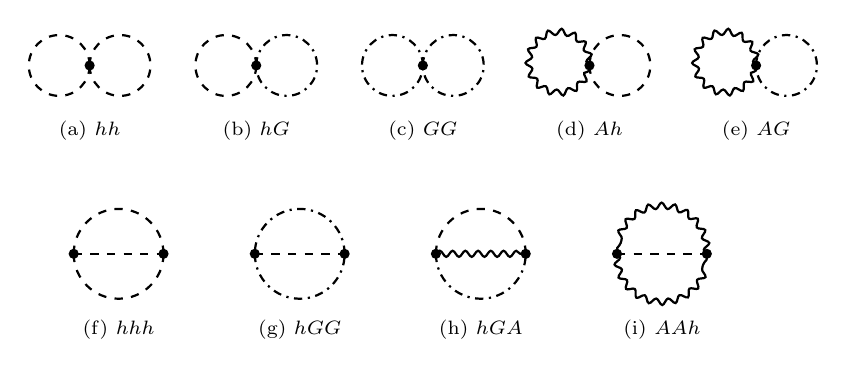
\begin{tikzpicture}[scale=0.92]
\foreach \x/\a/\b/\lbl in {0/scalar/scalar/{(a) $hh$}, 2.3/scalar/gold/{(b) $hG$}, 4.6/gold/gold/{(c) $GG$},
    6.9/photon/scalar/{(d) $Ah$}, 9.2/photon/gold/{(e) $AG$}} {
  \begin{scope}[shift={(\x,0)}]
    \eight{\a}{\b}
    \node[slab] at (0,-0.9) {\lbl};
  \end{scope}}
\begin{scope}[shift={(0.4,-2.6)}]
\foreach \x/\t/\m/\bo/\lbl in {0/scalar/scalar/scalar/{(f) $hhh$}, 2.5/gold/scalar/gold/{(g) $hGG$},
    5.0/scalar/photon/gold/{(h) $hGA$}, 7.5/photon/scalar/photon/{(i) $AAh$}} {
  \begin{scope}[shift={(\x,0)}]
    \sunset{\t}{\m}{\bo}
    \node[slab] at (0,-1.05) {\lbl};
  \end{scope}}
\end{scope}
\end{tikzpicture}
\caption{Landau ゲージの2ループの真空の図（1粒子既約）。破線は $h$、一点鎖線は Goldstone ボソン $G$、波線はゲージ場 $A$（横波）。(a)〜(c) は4点の頂点 $\lambda(h^2+G^2)^2/4$、(d)、(e) は $\frac12e^2A^2(h^2+G^2)$、(f)、(g) は $\lambda\phi h(h^2+G^2)$、(h) は微分を含む $eA_\mu(G\partial^\mu h-h\partial^\mu G)$、(i) は $e^2\phi A^2h$ の頂点による。ゴーストの日の出型の図は、ゴーストと $h$ の結合が $\xi$ に比例するので Landau ゲージでは0である。式~\eqref{eq:V2} の1行目が (a)〜(c)、(f)、(g)、2行目が (d)、(e)、(h)、(i) である。}
\label{fig:v2diag}
\end{figure}

\paragraph{極と対抗項。}$\MSbar$ の $V_2$ は、2ループの図に、1ループの $\MSbar$ の対抗項を1ループの図に挿入した項を加えた和の $\epsilon^0$ の係数である。Landau ゲージの1ループの対抗項は1ループのノートの値の $\xi=0$ で、$\delta Z_\Phi=3e^2/(K\epsilon)$、$\delta Z_A=-e^2/(3K\epsilon)$、$\delta_{m^2}=(4\lambda-3e^2)/(K\epsilon)$、$\delta_\lambda=(10\lambda-6e^2+3e^4/\lambda)/(K\epsilon)$ である。これらを場に依存する質量に入れると、挿入の項は
\begin{equation}
\frac1{K^2}\Bigl[\frac{X_h}2\mathbf A(x_h)+\frac{X_G}2\mathbf A(x_G)+\frac{3-2\epsilon}2\cdot\frac{10e^2x_A}{3\epsilon}\mathbf A(x_A)\Bigr],\qquad
X_{h,G}=\frac1\epsilon\Bigl[-m^2(4\lambda-3e^2)+c_{h,G}\lambda\phi^2\Bigl(10\lambda-3e^2+\frac{3e^4}\lambda\Bigr)\Bigr]
\label{eq:ct}
\end{equation}
になる（$c_h=3$、$c_G=1$。\ref{app:v2}）。ゲージ場の項は $x_A(\delta Z_\Phi-\delta Z_A)$ で、$Z_eZ_A^{1/2}=1$ から $x_A$ の繰り込みは場の $Z_\Phi$ だけになる。2ループの図と式~\eqref{eq:ct} の和の極は
\begin{equation}
\begin{aligned}
\frac1{\epsilon^2}:\ &\frac{3e^2-4\lambda}2m^4+(3e^4-6e^2\lambda+14\lambda^2)m^2\phi^2-\frac52(e^6+3e^4\lambda-3e^2\lambda^2+10\lambda^3)\phi^4,\\
\frac1\epsilon:\ &-2e^2m^4+\Bigl(\frac{11}4e^4+8e^2\lambda-6\lambda^2\Bigr)m^2\phi^2+\Bigl(\frac{13}3e^6-\frac{23}4e^4\lambda-7e^2\lambda^2+16\lambda^3\Bigr)\phi^4
\end{aligned}
\label{eq:poles}
\end{equation}
で（$1/K^2$ を除く）、$\phi^2$ の多項式（局所的）になり、2ループの対抗項（$\delta_\lambda$、$\delta_{m^2}$、$\delta Z_\Phi$ の2ループの部分と真空のエネルギー）で消える。$A(x)$、$I$ を含む非局所的な極が残らないことが、図と1ループの対抗項の整合の検算になる（手順 (1)）。$1/\epsilon^2$ の係数は1ループの量で決まり、$1/\epsilon$ の係数は2ループの $\beta$ 関数と場の異常次元を与える（手順 (2)、第~\ref{sec:rg} 節）。

\subsection{2ループの繰り込み群}\label{sec:rg}

$V_0$ に場によらない真空のエネルギー $\Lambda$ を加え、$V_0=\Lambda-\frac12m^2\phi^2+\frac14\lambda\phi^4$ とする。有効ポテンシャルは尺度 $Q$ によらず、
\begin{equation}
\Bigl[Q\frac{\partial}{\partial Q}+\beta_\lambda\frac{\partial}{\partial\lambda}+\beta_e\frac{\partial}{\partial e}+\beta_{m^2}\frac{\partial}{\partial m^2}+\beta_\Lambda\frac{\partial}{\partial\Lambda}-\gamma\,\phi\frac{\partial}{\partial\phi}\Bigr]V=0
\label{eq:rge}
\end{equation}
を満たす（$\beta_X=\dd X/\dd\ln Q$、$\dd\phi/\dd\ln Q=-\gamma\phi$）。$\beta$ 関数と $\gamma$ は、Machacek--Vaughn の一般の式~\cite{mv83} に Luo--Wang--Xiao の修正~\cite{lwx03} を加えたものから求める。一般の式は実のスカラー $\phi_a$ で書かれているので、$\Phi=(\phi_1+i\phi_2)/\sqrt2$ とし、4点の結合を $\lambda_{abcd}=2\lambda(\delta_{ab}\delta_{cd}+\delta_{ac}\delta_{bd}+\delta_{ad}\delta_{bc})$、生成子を $\theta=\bigl(\begin{smallmatrix}0&-i\\ i&0\end{smallmatrix}\bigr)$（$C_2(S)=1$、$S_2(S)=2$、$C_2(G)=0$）とする。$m^2$ と $\Lambda$ は、伝播しないダミーのスカラー $\hat d$ を使い、$\lambda_{ab\hat d\hat d}=-2m^2\delta_{ab}$、$\lambda_{\hat d\hat d\hat d\hat d}=24\Lambda$ の4点の結合として入れる~\cite{lwx03}（\ref{app:rg}）。$X=X^{(1)}/K+X^{(2)}/K^2$ と書くと、
\begin{equation}
\begin{aligned}
\beta_\lambda^{(1)}&=20\lambda^2-12e^2\lambda+6e^4,&
\beta_\lambda^{(2)}&=-240\lambda^3+112e^2\lambda^2+\frac{316}3e^4\lambda-\frac{208}3e^6,\\
\beta_{m^2}^{(1)}&=m^2(8\lambda-6e^2),&
\beta_{m^2}^{(2)}&=m^2\Bigl(-40\lambda^2+64e^2\lambda+\frac{86}3e^4\Bigr),\\
\beta_e^{(1)}&=\frac{e^3}3,&\beta_e^{(2)}&=4e^5,\\
\beta_\Lambda^{(1)}&=m^4,&\beta_\Lambda^{(2)}&=8e^2m^4,\\
\gamma^{(1)}&=-3e^2,&\gamma^{(2)}&=4\lambda^2+\frac{10}3e^4\qquad(\text{Landau ゲージ})
\end{aligned}
\label{eq:rg}
\end{equation}
である。$\beta$ 関数はゲージによらず、$\gamma$ は Landau ゲージの値である。1ループの部分は1ループのノートの対抗項と同じで、$\lambda^3$ の係数は $O(N)$ 模型の $-12(3N+14)$ の $N=2$ の値である。$V_0$ は $e$ を含まないので、$\beta_e^{(2)}$ は $1/K^2$ の次数の式~\eqref{eq:rge} には現れない。

$V_0$ の裸の量は $m_0^2\phi_0^2$ と $\lambda_0\phi_0^4$ の組でしか現れないので、極~\eqref{eq:poles} からは $\beta_\lambda-4\lambda\gamma$、$\beta_{m^2}-2m^2\gamma$、$\beta_\Lambda$ の組だけが決まる。$L$ ループの単純極の留数の $2L$ 倍がこれらを与える（\ref{app:rg}）。式~\eqref{eq:rg} から
\begin{equation}
\beta_\lambda^{(2)}-4\lambda\gamma^{(2)}=-\frac43(52e^6-69e^4\lambda-84e^2\lambda^2+192\lambda^3),\qquad
\beta_{m^2}^{(2)}-2m^2\gamma^{(2)}=2m^2(11e^4+32e^2\lambda-24\lambda^2)
\label{eq:rgcomb}
\end{equation}
であり、これは極~\eqref{eq:poles} の $1/\epsilon$ の係数の $\phi^4$、$\phi^2$ の項の $-16$ 倍、$8$ 倍に等しい（手順 (2) で確かめる）。

\subsection{最小点の Goldstone ボソン}\label{sec:goldstone}

木の最小点 $\phi=v_0$（$v_0^2=m^2/\lambda$）では $G\equiv x_G=-m^2+\lambda\phi^2$ が0になり、$G$ の小さいところで $V_2$ は解析的でない。Martin~\cite{martin14} に従って、$G\to0$ での主要な項を取り出す。$G$ の線の運動量が $\sqrt G$ 程度の領域では、残りの部分図は運動量0の $G$ の自己エネルギーになり、
\begin{equation}
V_2=\frac12\Delta_1A(G)+(\text{$G$ の0次と1次の項})+O(G^2\ln^2G),\qquad
\Delta_1=3\lambda A(x_h)+e^2\bigl[3A(x_A)+2x_A\bigr]
\label{eq:soft}
\end{equation}
となる。$\Delta_1$ は $h$ と $A$ のループによる $G$ の運動量0の自己エネルギーで、$h$ の4点の頂点の $\lambda A(x_h)$、$h$ と $G$ の泡の $(\lambda^{hGG})^2A(x_h)/x_h=2\lambda A(x_h)$（$x_h=2\lambda\phi^2$ のとき）、$A$ の4点の頂点の $e^2(3-2\epsilon)\mathbf A(x_A)$ の有限部分 $e^2[3A(x_A)+2x_A]$ からなる。$AGh$ の頂点は、$G$ の運動量が0のとき横波の射影で0になる。$\Delta_1$ は、$V_1$ から $G$ の項を除いたものの $\phi^{-1}\partial/\partial\phi$ に等しい。式~\eqref{eq:soft} から、$\phi^{-1}\partial V_2/\partial\phi$ は $\lambda\Delta_1\ln G$ を含み、木の最小点で対数で発散する。3ループ以上では $1/G$ の冪で発散する~\cite{martin14}。また、ループの補正を入れた最小点では $G\approx-\Delta_1/K$ である。基準点（$Q=1$）では $\Delta_1>0$ なので最小点で $G<0$ になり、$V_1$ の $f(G)=\frac14G^2(\ln G-\frac32)$ が虚部を持つ。

Martin の再和は、$G$ の線の輪に自己エネルギーの挿入を並べた図を全次数で足して $f(G)$ を $f(G+\Delta)$ に置き換えるもので、2ループまでの $V$ に対しては
\begin{equation}
\hat V=V+\frac1K\Bigl[f\Bigl(G+\frac{\Delta_1}K\Bigr)-f(G)\Bigr]-\frac1{K^2}\,\frac{\Delta_1}2A(G)
\label{eq:vhat}
\end{equation}
である（Goldstone ボソンは1個）。$\hat V$ の最小化の条件は、$G$ を含まない形
\begin{equation}
-m^2+\lambda v^2=-\frac1K\hat\Delta_1-\frac1{K^2}\hat\Delta_2,\qquad
\hat\Delta_1=3\lambda A(h)+e^2\bigl[3A(x_A)+2x_A\bigr],\qquad h=2\lambda v^2,\quad x_A=e^2v^2
\label{eq:mincond}
\end{equation}
に書ける~\cite{martin14}。$\hat\Delta_2$ は、$\phi^{-1}\partial V_2/\partial\phi$ から $\lambda\Delta_1\ln G$ を除いて $G\to0$ とし、$3\lambda A(x_h)=3\lambda A(h)+3\lambda G\ln h+\cdots$ の $G$ を $-\hat\Delta_1/K$ で置き換えた $-3\lambda\hat\Delta_1\ln h$ を加えたものである。本模型では
\begin{equation}
\begin{aligned}
v^4\hat\Delta_2={}&-\frac{15}4h^2I(h,h,h)-\frac12h^2I(0,0,h)+\frac32h(h+x_A)I(0,x_A,h)\\
&-\frac{7h^3-50h^2x_A+148hx_A^2-216x_A^3}{4(h-4x_A)}I(x_A,x_A,h)+\frac{13h^3-59h^2x_A+76hx_A^2-180x_A^3}{2(h-4x_A)}A(h)\\
&-\frac{2h^2-11hx_A+18x_A^2}{h-4x_A}A(h)A(x_A)+\frac{7h^2-36hx_A+56x_A^2}{4(h-4x_A)}A(x_A)^2+\frac{x_A(3h^2+44hx_A-188x_A^2)}{3(h-4x_A)}A(x_A)\\
&-\frac{42h^4-180h^3x_A+51h^2x_A^2+172hx_A^3-520x_A^4}{6(h-4x_A)}
\end{aligned}
\label{eq:dh2}
\end{equation}
である（手順 (3)、\texttt{results/goldstone.m}）。最小点での $\hat V$ の値は、$m^2$ と $G$ を消して
\begin{equation}
\hat V_{\min}=\Lambda-\frac\lambda4v^4+\frac1K\Bigl[f(h)+3f_V(x_A)-\frac{v^2}2\hat\Delta_1\Bigr]+\frac1{K^2}\Bigl[V_2\big|_{G=0,\,x_h=h}-\frac{v^2}2\hat\Delta_2-\frac12\hat\Delta_1A(h)\Bigr]
\label{eq:vmin}
\end{equation}
となる（$f_V(x)=\frac14x^2(\ln x-\frac56)$）。$m^2$ を固定するなら、木の最小点のまわりの $\hbar$ 展開~\cite{pr11} $v=v_0+v_1/K+v_2/K^2$、$V_{\min}=V_0+V_1/K+[V_2-V_1'^2/(2V_0'')]/K^2$（右辺は $v_0$ での値）でもよい。$V_{\min}$ のこの式は $G=0$ でも有限である。$v_2$ では $V_2'$ と $v_1V_1''$ の $\ln G$ が打ち消す。

最小点での曲率 $\partial^2V/\partial\phi^2$ は、1ループですでに $f''(G)(2\lambda\phi)^2=2\lambda^2\phi^2\ln G$ を含む。再和しても $\ln(G+\Delta)$ の形で残り、$G+\Delta$ は最小点で0に近い。これは質量0の Goldstone ボソンのループが運動量0のスカラーの自己エネルギーに与える赤外の対数で、曲率はスカラーの質量の良い近似にならない。そこで、計画した「曲率」は求めず、スカラーの質量には自己エネルギーの運動量依存（極の質量）が要るとして本ノートの範囲の外とした。

\subsection{背景場の $R_\xi$ ゲージと Nielsen 恒等式}\label{sec:rxi}

背景場の $R_\xi$ ゲージでは、ゲージ固定を $F=\partial\!\cdot\!A-\xi e\phi G$ とする（1ループのノートの $R_\xi$ ゲージの $v$ を背景場 $\phi$ に置き換えたもの）。$A$ と $G$ の混合は打ち消し、質量の2乗は $h$ が $H\equiv x_h$、横波が $Z\equiv x_A$、Goldstone ボソンが $Z_+\equiv G+\xi Z$、縦波の $\xi$ の極とゴーストが $\eta\equiv\xi Z$ になる。1ループは $V_1=f(H)+3f_V(Z)+f(G+\xi Z)-f(\xi Z)$ で、$G=0$ では Landau ゲージの値に一致する。Martin と Patel~\cite{mp18} は、ゲージ固定を $F=\partial\!\cdot\!A-\tilde\xi e\phi G$ と $\xi$ に一般化した $\MSbar$ の $V_2$ を一般の理論と本模型で求め、$\tilde\xi=\xi$ で
\begin{equation}
\begin{aligned}
\phi^2V_2^{(\xi)}={}&\Bigl(HZ-\frac{H^2}4-3Z^2\Bigr)I(H,Z,Z)+\Bigl[(H+Z-G)\eta-\frac{\eta^2}2-\frac{\lambda_K(G,H,Z)}2\Bigr]I(H,Z,Z_+)\\
&-\frac{(H-G)^2}4I(H,Z_+,Z_+)+\Bigl[\frac{(H+\eta-Z)^2}2-2\eta H\Bigr]I(H,Z,\eta)+\frac{(H-Z_+)^2}2I(H,\eta,Z_+)\\
&+\Bigl(\eta H-\frac{\eta^2}2-\frac{H^2}4\Bigr)I(H,\eta,\eta)-\frac34(H-G)^2I(H,H,H)+\Bigl(\frac H4-\frac Z2\Bigr)A(Z)^2\\
&+\Bigl(\frac H4-\frac\eta2\Bigr)A(\eta)^2+\frac38(H-G)\bigl[A(Z_+)^2+A(H)^2\bigr]+\frac{H+2Z-\eta-G}2A(Z)A(Z_+)\\
&+\frac{Z_+-H}2A(\eta)A(Z_+)+\frac{Z+\eta-H}2A(Z)A(\eta)+\frac{3Z-H+G}2A(H)A(Z)\\
&+\frac{H+2Z-G}4A(H)A(Z_+)+\frac{H-Z-G}2A(H)A(\eta)+Z\Bigl(G+H+\frac{2Z}3\Bigr)A(Z)\\
&+3Z^2A(H)+Z^2A(Z_+)-Z^2(2Z+H)
\end{aligned}
\label{eq:V2rxi}
\end{equation}
を与えた（$G=H-2\lambda\phi^2$、$Z=e^2\phi^2$。$\xi=0$ で式~\eqref{eq:V2} になる）。$\xi$ と $\tilde\xi$ は異なる割合で走り、背景場の走り $\beta_\phi=\dd\phi/\dd\ln Q$ も Landau ゲージと異なる~\cite{mp18}：
\begin{equation*}
\beta_\xi^{(1)}=-\frac23e^2\xi,\qquad \beta_{\tilde\xi}^{(1)}=2e^2\Bigl(\xi-\tilde\xi-\frac{10}3\Bigr)\tilde\xi,\qquad
\beta_\phi=\frac{(3-\xi+2\tilde\xi)e^2}K\phi+\frac{e^4(-\frac{10}3+2\tilde\xi+2\xi\tilde\xi)-4\lambda^2}{K^2}\phi.
\end{equation*}$\tilde\xi=\xi$ は繰り込み群で保たれないので、繰り込み群の検算には $\tilde\xi\ne\xi$ の $V_1$ が要る。$\tilde\xi-\xi$ の1次までは、上の $V_1$ の Goldstone ボソン、縦波、ゴーストの部分を $f(G+(2\tilde\xi-\xi)Z)+f(\xi Z)-2f(\tilde\xi Z)$ とすればよい。

\paragraph{Nielsen 恒等式。}有効ポテンシャルの $\xi$ 依存は場の再定義で吸収でき、極値の値はゲージによらない~\cite{nielsen75,ahnote}。$m^2$ を固定した $\hbar$ 展開では、
\begin{equation}
V_{\min}=V_0(v_0)+\frac1KV_1(v_0)+\frac1{K^2}N,\qquad N=V_2(v_0)-\frac{V_1'(v_0)^2}{2V_0''(v_0)}
\label{eq:N}
\end{equation}
で（$v_0^2=m^2/\lambda$、$G=0$）、$V_1(v_0)$ は $\xi$ によらない。背景場の $R_\xi$ ゲージでは $V_1'(v_0)=v_0[\hat\Delta_1+\lambda A(\xi Z)]$ が $\xi$ による。$N$ が $\xi$ によらないことは、
\begin{equation}
V_2^{(\xi)}(v_0)=V_2^{(0)}(v_0)+\frac12\hat\Delta_1A(\xi Z)+\frac14\lambda A(\xi Z)^2
\label{eq:nielsen2}
\end{equation}
と同じである（手順 (4) で記号として確かめる）。$\xi\ne0$ では最小点の Goldstone ボソンの質量 $G+\xi Z$ が正なので、手順 (3) の赤外の問題は起きない。

\paragraph{Fermi ゲージ。}$\tilde\xi=0$ では、$A$ の縦波と $G$ が $-e\phi A\!\cdot\!\partial G$ で混ざる。この組の質量の2乗は $x^2-Gx+\xi ZG=0$ の根 $Z_\pm=\frac12[G\pm\sqrt{G(G-4\xi Z)}]$ で、ゴーストは質量を持たない。$0<G<4\xi Z$ では $Z_\pm$ は複素共役の組になり、$G<0$ では $Z_-<0$ で $V$ は複素数になる。Martin--Patel は、一般の $(\xi,\tilde\xi)$ の $V_2$ を論文の付属の電子ファイルで与えた~\cite{mp18}。木の最小点の近くでは、$G$ と縦波の組の伝播関数が $1/k^4$ の極を持つ。そのため Espinosa--Garny--Konstandin~\cite{egk16} が示したとおり、$f(Z_+)+f(Z_-)\simeq-\frac14\xi ZG[\ln(\xi Z|G|)-3]$ から $V_1'$ が $\ln|G|$ で発散する（1ループのノートの手順 (7)）。$V_1'(v_0)$ と $V_2(v_0)$ がどちらも発散するので、Fermi ゲージでは式~\eqref{eq:N} の $\hbar$ 展開が作れない。

\subsection{Coleman--Weinberg の模型の次の次数}\label{sec:cwnlo}

$m^2=0$ では木の最小点は原点で、1ループの補正が対称性を破る（1ループのノートの手順 (8)）。$\lambda\sim e^4/K$ と数え、$L=\ln(e^2\phi^2/Q^2)$、$V=\phi^4W(L)$ と書く。主要な次数は $W_0=\frac\lambda4+\frac{3e^4}{4K}(L-\frac56)$ で、最小点は $L_0=\frac13-\frac{K\lambda}{3e^4}$、最小値は $V_{\mathrm{LO}}=-\frac{3e^4}{8K}v_0^4$、曲率の比は $R\equiv V''(v)/(e^2v^2)=6e^2/K=3e^2/(8\pi^2)$ である。相対 $e^2/K$ の次の次数には二つの項が入る。一つ目は1ループの $\lambda$ の1次の項で、Landau ゲージにはなく、背景場の $R_\xi$ ゲージでは $f(G+\xi Z)-f(\xi Z)\simeq\frac12GA(\xi Z)$ から $\frac{\lambda\xi e^2}{2K}(L+\ln\xi-1)$ である。二つ目は $V_2$ の $\lambda\to0$ の値で（$\lambda$ を含む項は $\lambda\ln\lambda$ の大きさで、次の次の次数）、
\begin{equation}
W\supset\frac{e^6}{K^2}P_\xi(L),\qquad P_\xi(L)=\frac52L^2-\frac{31}3L+\frac{71}6+\frac32\xi\Bigl(L-\frac13\Bigr)(L+\ln\xi-1)
\label{eq:Pxi}
\end{equation}
である（$\xi=0$ が Landau ゲージ）。$\xi=0$ の多項式は Andreassen--Frost--Schwartz~\cite{afs15} の式 (5.20) の $\xi=0$ と Espinosa--Garny--Konstandin~\cite{egk16} の式 (14) に一致する。$\xi$ の項では、$I(0,Z,\xi Z)$ の二重対数が打ち消して多項式と $\ln\xi$ だけが残る。これは $\lambda\to0$ での2ループの Nielsen 恒等式 $\partial_\xi V_2=C_1\partial_\phi V_1$（$C_1=\frac{e^2\phi}{2K}\ln(\xi Z/Q^2)$、1ループのノートの $C_{\mathrm{bg}}$ の $G\to0$）を積分したものである。

最小値は停留値なので、次の次数の項を $L_0$ で評価すればよい。1ループの $\lambda\xi$ の項（$\lambda=\frac{e^4}K(1-3L_0)$）と $P_\xi-P_0$ が $L_0$ で打ち消し、
\begin{equation}
V_{\min}=-\frac{3e^4}{8K}v_0^4\Bigl[1-\frac{8e^2}{3K}P_0(L_0)\Bigr],\qquad v_0^2=\frac{Q^2}{e^2}e^{L_0}
\label{eq:cwvmin}
\end{equation}
はゲージによらない。$\mu=M_A$ にとる $L_0=0$（$\lambda=e^4/K$）では $V_{\min}=V_{\mathrm{LO}}(1-\frac{284}9\frac{e^2}K)$ である。一方、曲率の比は、$W'$ と $W''$ を $L_0$ で評価して
\begin{equation}
R=\frac{6e^2}K\Bigl[1+\frac{e^2}Kr_1\Bigr],\qquad r_1=\frac29\bigl[30L_0-47+9\xi(L_0+\ln\xi)\bigr]
\label{eq:cwR}
\end{equation}
となり、ゲージに依存する。1ループだけでは $r_1=\frac23\xi(1-3L_0)$ で（1ループのノートの式の背景場の $R_\xi$ ゲージ）、$V_2$ を加えると $\xi$ 依存が $2\xi(L_0+\ln\xi)$ に変わるが消えない。Nielsen 恒等式から、最小点の曲率は $\dd V''(v)/\dd\xi=2C'V''$、最小点は $\dd v/\dd\xi=-C$ で動くので $\dd\ln R/\dd\xi=2C'+2C/v$ となり、$C_1$ を入れると $\frac{2e^2}K(L_0+\ln\xi+1)$ で、$\dd r_1/\dd\xi$ に一致する。曲率は運動量0の2点関数で、極の質量ではないので、ゲージによらない質量の比には自己エネルギーの運動量依存が要る。

\section{検算の計画}\label{sec:plan}

第~\ref{sec:results} 節の量と、これから求める量を、どの手段で計算して突き合わせるかを表~\ref{tab:plan} に示す。手計算（付録）を基準とし、ツールの出力がそれと一致するかを確かめる。ツールの版と配置は計算環境の記録~\cite{env} にあり、1ループのノートと同じものを使う。

\begin{table}[tbp]
\centering\small
\caption{各量と、それを計算して突き合わせる手段。「—」はその手段を使わないことを表す。}
\label{tab:plan}
\begin{tabularx}{\linewidth}{>{\raggedright\arraybackslash}p{3.3cm}>{\raggedright\arraybackslash}p{1.3cm}>{\raggedright\arraybackslash}X>{\raggedright\arraybackslash}p{2.6cm}>{\raggedright\arraybackslash}p{2.4cm}}
\toprule
\textbf{量} & \textbf{手計算} & \textbf{FeynArts、FeynCalc、Kira} & \textbf{数値（TSIL、AMFlow）} & \textbf{その他} \\
\midrule
(1) Landau ゲージの $V_2$ \eqref{eq:V2} & \ref{app:v2} & 10個の真空の図、対抗項の挿入、Martin の式と記号として & $I(x,y,z)$ & — \\
(2) 2ループの繰り込み群 \eqref{eq:rg} & \ref{app:rg} & 極 \eqref{eq:poles} から $\beta$、$\gamma_\phi$ & $\dd V/\dd\ln Q$ & 一般の公式~\cite{mv83,lwx03} \\
(3) Goldstone の赤外の再和 & \ref{sec:goldstone} & — & 最小点、$V_{\min}$ & 文献~\cite{martin14,eek14,pr11} \\
(4) 背景場の $R_\xi$ と Fermi ゲージの $V_2$ \eqref{eq:V2rxi}、Nielsen 恒等式 & \ref{sec:rxi} & 背景場の $R_\xi$ ゲージで図から & $V_{\min}$ の $\xi$ によらないこと、固定次数の最小値 & Martin--Patel~\cite{mp18}、文献~\cite{egk16} \\
(5) CW の模型の次の次数（最小値と曲率の比） & \ref{sec:cwnlo} & — & 全体のポテンシャルを最小化（Landau、背景場の $R_\xi$） & 文献~\cite{afs15,egk16} \\
(6) 有限温度の次の次数 & 後で & — & $T_c$、$\phi_c/T_c$ & DRalgo~\cite{dralgo} \\
(7) 3次元の格子との比較（任意） & 後で & — & 3次元のパラメータ & 文献~\cite{kklp98} \\
\bottomrule
\end{tabularx}
\end{table}

\paragraph{一致の基準。}記号の比較は、極と有限部分の差が記号として0になることを求める。$I(x,y,z)$ のように閉じた形の関数は、独立な二つの数値（TSIL の解析式と AMFlow の微分方程式）が倍精度の範囲で一致することを求める。ゲージによらないはずの量は、複数の $\xi$ とゲージで同じ値になることを、$\hbar$ の次数ごとに求める。文献との比較は、文献の数を写すのでなく、本ノートの模型と規格化で計算した量で行う。

\paragraph{手順。}次の順に進める。(1) Landau ゲージの $V_2$：手計算の式~\eqref{eq:V2} を、FeynArts で作った2ループの真空の図（FeynCalc で縮約と部分分数、Kira で簡約）と1ループの対抗項の挿入から求めた値と記号として比べる。$I(x,y,z)$ の数値を TSIL と AMFlow で比べる。(2) 2ループの繰り込み群：一般の公式~\cite{mv83,lwx03} から2ループの $\beta_\lambda$、$\beta_{m^2}$、$\beta_e$ と Landau ゲージの $\gamma_\phi$ を求め、極~\eqref{eq:poles} との整合と、$\dd V/\dd\ln Q=O(\hbar^3)$ を記号として確かめる。(3) Goldstone の赤外の問題：最小点で $x_G\sim\hbar$ となり、$V_2$ の微分に $\ln x_G$ が現れることを示し、再和~\cite{martin14,eek14} で最小点と $V_{\min}$ を2ループの精度で求める（計画の時点では曲率も挙げたが、最小点で赤外の対数を持つので除いた。第~\ref{sec:goldstone} 節）。(4) 一般のゲージ：Martin--Patel の一般のゲージ固定の式~\cite{mp18} を本模型に当てはめて、背景場の $R_\xi$ ゲージと Fermi ゲージの $V_2$ を作り、一つのゲージでは図からも計算する。極値の値が $O(\hbar^2)$ まで $\xi$ によらないことを、1ループのノートの手順 (7) の $\hbar$ の尺度の方法で確かめる。Fermi ゲージの赤外の問題~\cite{egk16} は手順 (3) の再和と組み合わせる（実際には、Fermi ゲージでは木の最小点で $V_1'$ と $V_2$ が対数で発散して式~\eqref{eq:N} の $\hbar$ 展開が作れないので、Martin--Patel の一般のゲージの $V_2$ で固定した次数の最小値を数値で求め、ゲージによらない値と比べた。再和はしていない）。(5) CW の模型：$m^2=0$、$\lambda\sim e^4/K$ と数えて、最小値と曲率の比 $M_h^2/M_A^2=V''(v)/(e^2v^2)$ を相対 $e^2/K$ まで求め、1ループのノートの手順 (8) のゲージ依存がどうなるかを確かめる（計画の時点では比のゲージ依存が消えると見込んだが、消えるのは最小値で、曲率の比は Nielsen 恒等式どおり次の次数でもゲージに依存した。第~\ref{sec:cwnlo} 節）。Andreassen--Frost--Schwartz~\cite{afs15} とは、本ノートの模型で計算した量で比べる。(6) 有限温度：DRalgo の NLO の次元簡約と3次元の2ループのポテンシャルで、$\lambda\sim e^3$ と数えて $T_c$ と $\phi_c/T_c$ を次の次数までゲージによらない展開で求め~\cite{el20}、1ループのノートの手順 (10) と比べる。(7) 3次元の U(1)＋ヒッグスの格子の結果~\cite{kklp98} と、本ノートで求めた3次元のパラメータで比べる（任意）。

\section{検算}\label{sec:checks}

第~\ref{sec:plan} 節の手順を順に行う。スクリプトはすべて \texttt{Src/} にあり、手順 (1) は \texttt{run\_v2\_check.sh}（AMFlow を含めて約40分）、手順 (2) は \texttt{run\_rg2\_check.sh}（数秒）、手順 (3) は \texttt{run\_goldstone\_check.sh}（約15秒）、手順 (4) は \texttt{run\_rxi\_check.sh}（数分）と \texttt{run\_fermi\_check.sh}（約30秒）、手順 (5) は \texttt{run\_cw\_check.sh}（数分）で再実行できる。

\paragraph{手順 (1)：Landau ゲージの $V_2$。}三つのスクリプトで確かめた。一つ目は \texttt{v2\_landau\_feyncalc.wl} である。(a) 1ループのノートの FeynRules の模型（\texttt{models/abelian\_higgs/Src/generated/AbelianHiggs\_FA}）を FeynCalc の FeynArts のパッチを当てて写し、Goldstone ボソンの質量を $\sqrt\xi M_A$ から独立な記号 $M_G$ に替えた（Landau ゲージの背景場での質量 $x_G$）。FeynArts の \texttt{CreateTopologies[2, 0 -> 0]} から1粒子既約な真空の図を作ると10個で、ゴーストの図は \texttt{GaugeXi -> 0} で0になった（残りが図~\ref{fig:v2diag} の9個）。背景場は模型の \texttt{vev} を $\phi$ と読み替えた（結合は $\lambda\,\texttt{vev}$、$e^2\texttt{vev}$ の形で、質量の記号とは独立である）。(b) FeynCalc で Lorentz の添字を縮約し、\texttt{ApartFF} で横波の射影の $1/k^2$ を部分分数に分け、\texttt{FCLoopFindTopologies}、\texttt{FCLoopFindTopologyMappings}、\texttt{FCLoopBasisFindCompletion} で10個の積分族と23個の積分にまとめた。(c) Kira 3.1 で、点や分子のない積分（日の出型と1ループの積の積分）を優先したマスター積分に簡約した。18個のマスター積分はすべて点も分子もなく、係数の分母に $D$ を含む因子はなかった（$\epsilon$ の極を持つ係数がない）。(d) Minkowski の積分を Euclid の太字の積分 \eqref{eq:bold} に直し（1ループの積は $-\mathbf A\mathbf A$、日の出型は $+\mathbf I$。\ref{app:details}）、対抗項の挿入~\eqref{eq:ct} を加えて $\epsilon$ で展開した。$1/\epsilon^2$ と $1/\epsilon$ の係数には $A$、$\Aeps$、$I$ を含む項が残らず、極は式~\eqref{eq:poles} の多項式になった。有限部分は、$\Aeps(x)=-\frac12[x(1+\zeta_2)+A(x)^2/x]$ を使うと、式~\eqref{eq:V2} と17個の単項式（$I$ の7通り、$A$ の積と1次の項、定数）のすべてで記号として一致した。式~\eqref{eq:V2} を \texttt{results/v2\_landau.m} に書き出した。

二つ目と三つ目は $I(x,y,z)$ の数値である。$\phi=2$（木の最小点、$x_G=0$）と $\phi=3$ で $V_2$ に要る11個の質量の組について、TSIL 1.46~\cite{tsil} の \texttt{TSIL\_I2}（解析式、\texttt{v2\_tsil.c}）と、AMFlow 2.0~\cite{amflow} の補助質量の流れ（Kira で簡約、30桁、\texttt{v2\_amflow.wl}）で求めた。AMFlow の太字の積分の $\epsilon^{-2}$、$\epsilon^{-1}$ の係数は式~\eqref{eq:bold} と27桁以上一致し、$I$ は TSIL と相対 $2\times10^{-15}$ 以内で一致した（\texttt{v2\_numeric.py}、表~\ref{tab:v2num}）。基準点の木の最小点 $\phi=2$ では、$V_0=-3.125$、$V_1/K=0.0166095$、$V_2/K^2=-0.00251355$ で、2ループは1ループの15\%の大きさで符号が逆である（$\lambda=0.78$ の $hhh$ の日の出型が最も大きい）。$\phi=3$ では $V_2/K^2=0.0150405$ で、$V_1/K=0.705954$ の2\%である。二つの $I$ の組で求めた $V_2$ は相対 $9\times10^{-16}$ 以内で一致した。

\begin{table}[tbp]
\centering\small
\caption{基準点（$e=\frac12$、$\lambda=\frac{25}{32}$、$m^2=\frac{25}8$、$Q=1$）での Landau ゲージの有効ポテンシャルの各次数。$V_2/K^2$ は TSIL と AMFlow の $I$ で求めた値（\texttt{results/v2\_numeric.csv}）。}
\label{tab:v2num}
\begin{tabular}{rrrrr}
\toprule
$\phi$ & $V_0$ & $V_1/K$ & $V_2/K^2$（TSIL） & $V_2/K^2$（AMFlow） \\
\midrule
2 & $-3.125$ & $0.01660949$ & $-2.513548132989\times10^{-3}$ & $-2.513548132989\times10^{-3}$ \\
3 & $1.7578125$ & $0.70595449$ & $1.504050155047\times10^{-2}$ & $1.504050155047\times10^{-2}$ \\
\bottomrule
\end{tabular}
\end{table}

\paragraph{手順 (2)：2ループの繰り込み群。}二つのスクリプトで確かめた。一つ目は \texttt{rg2\_mv.wl} である。(a) Machacek--Vaughn の一般の式を、Luo--Wang--Xiao~\cite{lwx03} の式 (22)、(23)、(30)、(38)、(44)（Machacek--Vaughn の誤りを直したもの）の形で、実のスカラーの添字を持つテンソルとして Mathematica に実装した。$m^2$ と $\Lambda$ はダミーのスカラーの4点の結合として入れ、内部の和からダミーを除いた。(b) 実装の検算として、標準模型のヒッグス2重項（実のスカラー4個）に $U(1)_Y$ だけを残した場合（$g=0$、湯川結合 0、3世代のフェルミオンは $\kappa S_2(F)=5$ として真空偏極にだけ入る）を計算した。$\beta_\lambda$ と $\beta_{m^2}$ の1ループと2ループは、Luo--Xiao~\cite{lx03} の式 (9)〜(12) の $g'$ と $\lambda$ の項（$\lambda_{\mathrm{LX}}=2\lambda$、$g_1^2=\frac53g'^2$ で換算すると、$\beta_\lambda^{(2)}=-312\lambda^3+36g'^2\lambda^2+\frac{629}{24}g'^4\lambda-\frac{379}{48}g'^6$、$\beta_{m^2}^{(2)}=m^2(-60\lambda^2+24g'^2\lambda+\frac{557}{48}g'^4)$）と記号として一致した。式 (44) の $\lambda g^4$ の項で $g^4$ がどの項まで掛かるかは、PDF の文字からは読み取りにくい。$\Lambda^{SS}$、$A^\lambda$、$\bar A^\lambda$ の項まで括弧に入れる読み方がこの比較で正しいと確かめた。(c) 本模型の値を入れると式~\eqref{eq:rg} を得た（\texttt{results/rg2.m}）。$\beta$ のテンソルは $O(2)$ の対称な形を保つ（$\beta_{1122}=\beta_{1111}/3$ など）。(d) 式~\eqref{eq:rg} から作った $V_0$ の2ループの $\MSbar$ の対抗項（\ref{app:rg}）は、手順 (1) の図と対抗項の挿入の極~\eqref{eq:poles}（\texttt{results/v2\_landau.m}）を $1/\epsilon^2$ と $1/\epsilon$ の両方で記号として打ち消した。$1/\epsilon^2$ は1ループの関数だけで決まる極の整合の検算、$1/\epsilon$ は2ループの関数の組~\eqref{eq:rgcomb} と $\beta_\Lambda^{(2)}=8e^2m^4$ の検算である。(e) 式~\eqref{eq:rge} に $V_0+V_1/K+V_2/K^2$（$V_2$ は式~\eqref{eq:V2}）を入れ、$Q^2\partial A(x)/\partial Q^2=-x$、$Q^2\partial I(x,y,z)/\partial Q^2=A(x)+A(y)+A(z)-x-y-z$ を使うと、$1/K$ と $1/K^2$ の項はともに記号として0になった（$I$ は $Q$ の微分で消え、$A(x_h)$、$A(x_G)$、$A(x_A)$ の1次と多項式の恒等式になる）。$\gamma^{(2)}$ を除くと $\frac23(5e^4+6\lambda^2)\phi^2x_G$ が残るので、この検算は $\gamma^{(2)}$ にも感度を持つ。(d) と (e) は、図の極と有限部分（Martin の式）の両方が、一般の式の $\beta$、$\gamma$ と整合することを示す。

二つ目は \texttt{rg2\_numeric.py} で、繰り込み群の流れに沿った $V$ の変化を数値で見た。$Q=1$ で基準点の結合、$\phi=3$（$x_G>0$）、$\Lambda=0$ から始め、$\lambda$、$e$、$m^2$、$\Lambda$、$\phi$ を式~\eqref{eq:rg} で $Q=2$ まで流し（SciPy の DOP853、相対誤差 $10^{-13}$）、両端の $V$ を TSIL の $Q^2=1,4$ の $I$ で求めた。変化を見る組は、(a) $V_0+V_1/K$ と1ループの流れ、(b) $V_0+V_1/K+V_2/K^2$ と1ループの流れ、(c) $V_0+V_1/K+V_2/K^2$ と2ループの流れ、の三つである。次数を見るため、$m^2$ を固定して $\lambda\to s\lambda$、$e^2\to se^2$、$\phi\to\phi/\sqrt s$ と変えた。質量の2乗は変わらず、$V_0\propto1/s$、$V_1\propto1$、$V_2\propto s$ になるので、残る最初の次数は (a)、(b) で $s$、(c) で $s^2$ に比例するはずである。表~\ref{tab:rg2num} のとおり、$s$ を半分にするごとの比は (a) と (b) で2、(c) で4に近づく（ずれは次の次数の $O(s)$）。(b) は (a) の6割ほどで、(a) と同じく $s$ に比例する。$V_2$ を加えても、2ループの $\beta$ と $\gamma$ がなければ $1/K^2$ の変化は消えない。

\begin{table}[tbp]
\centering\small
\caption{繰り込み群の流れに沿った有効ポテンシャルの変化 $V(Q=2)-V(Q=1)$（\texttt{results/rg2\_numeric.csv}）。$Q=1$ で $\lambda=\frac{25}{32}s$、$e^2=\frac14s$、$m^2=\frac{25}8$、$\phi=3/\sqrt s$、$\Lambda=0$。(a) $V_0+V_1/K$ と1ループの流れ、(b) $V_0+V_1/K+V_2/K^2$ と1ループの流れ、(c) $V_0+V_1/K+V_2/K^2$ と2ループの流れ。最後の行は $s=\frac14$ と $\frac18$ の比。}
\label{tab:rg2num}
\begin{tabular}{rrrrr}
\toprule
$s$ & $V(Q=1)$ & (a) & (b) & (c) \\
\midrule
1 & $2.47881$ & $9.640\times10^{-2}$ & $5.568\times10^{-2}$ & $-5.938\times10^{-3}$ \\
$\frac12$ & $4.22910$ & $4.544\times10^{-2}$ & $2.652\times10^{-2}$ & $-1.391\times10^{-3}$ \\
$\frac14$ & $7.74096$ & $2.208\times10^{-2}$ & $1.295\times10^{-2}$ & $-3.363\times10^{-4}$ \\
$\frac18$ & $14.7703$ & $1.089\times10^{-2}$ & $6.399\times10^{-3}$ & $-8.267\times10^{-5}$ \\
\midrule
比 & & $2.028$ & $2.024$ & $4.068$ \\
\bottomrule
\end{tabular}
\end{table}

\paragraph{手順 (3)：最小点の Goldstone ボソン。}二つのスクリプトで確かめた。一つ目は \texttt{goldstone\_ir.wl} で、Martin~\cite{martin14} の付録の $I$ の公式（質量の2乗での微分の式 (A.23)、小さい $G$ での展開の式 (A.27)、(A.28)）を使う。(a) 式~\eqref{eq:V2} に $G$ の展開を入れると、$G\ln^2G$ の項はなく、$G\ln G$ の係数は $x_h=2\lambda\phi^2$、$x_A=e^2\phi^2$ で $\Delta_1/2$ に記号として等しかった（式~\eqref{eq:soft}）。(b) $\phi^{-1}\partial V_2/\partial\phi$ を (A.23) で求めて $G\to0$ とすると、$\ln^2G$ の項はなく、$\ln G$ の係数は $\lambda\hat\Delta_1$ に等しく、残りから式~\eqref{eq:dh2} を得た。(c) $m^2$ を固定した $\hbar$ 展開では、$V_2'$ の $\ln G$ と、$v_1V_1''$ の $\ln G$（$f''(G)=\frac12\ln G$ から）が打ち消し、$v_2$ は条件~\eqref{eq:mincond} を展開したものと記号として一致した。(d) 式~\eqref{eq:vmin} に $\hbar$ 展開の $v$ を入れると、$\hbar$ 展開の $V_{\min}$ と $1/K^2$ まで記号として一致した。(e) 条件~\eqref{eq:mincond} と $\hat V_{\min}$ に、手順 (2) の $\beta$、$\gamma$（$\beta_\Lambda$ を含む）で $Q\,\dd/\dd Q$ を作用させて $m^2$ を条件で消すと、$1/K$ と $1/K^2$ の項はともに0になった。(e) は $\hat\Delta_2$ の対数を含む部分の検算で、$Q$ によらない多項式の部分は次の数値で確かめる。

二つ目は \texttt{goldstone\_numeric.py} である。(a) 式 (A.23) は TSIL の $I$ の中心差分と相対 $4\times10^{-9}$（差分の誤差の大きさ）で、式 (A.27)、(A.28) は TSIL と $G^2\ln^2G$ 程度の差で一致した（$G=10^{-3}$〜$10^{-5}$）。(b) 図~\ref{fig:goldstone} は、$Q=1$ の基準点の木の最小点の近くで、$K\phi^{-1}\partial(V-V_0)/\partial\phi$ を $G$ の関数として描いたものである（\texttt{goldstone\_ir.wl} で解析的に微分し、$I$ に TSIL の値を入れた）。2ループの曲線は $\ln G$ について傾き $0.0591009$ で下がり続け、$\lambda\hat\Delta_1/K=0.0591008$ と一致する。再和した曲線は $G=10^{-10}$〜$10^{-6}$ で $1\times10^{-5}$ しか変わらない。なお、倍精度の TSIL の $I(G,G,x_h)$ は $G/x_h\lesssim10^{-7}$ で精度を落とす（式 (A.27) との差が $G=10^{-8}$ で $2\times10^{-6}$、$10^{-12}$ で $0.03$）ので、この図では差分を使わなかった。(c) $Q=1$ では最小点の $G\approx-\hat\Delta_1/K=-0.0756$ が負で、通常の $V$ は最小点で複素数になる。条件~\eqref{eq:mincond} と式~\eqref{eq:vmin} からは $v=1.978615$、$\hat V_{\min}=-3.112595$ を得て、$\hbar$ 展開の $v=1.978772$、$V_{\min}=-3.112735$ と $1/K^3$ の大きさの差で合う（1ループの $V_{\min}$ は $-3.108391$）。$V$ の最小点を数値で直接求めるため、$e$、$\lambda$、$m^2$ を同じ値のまま $Q=2$ で与えた点も使った。そこでは $\hat\Delta_1=-9.40$、最小点の $G\approx+0.0595$ で、$V$ は実数である。$\hat V$ と2ループの $V$ の最小点を数値で求め（5点の差分の導関数の根）、条件~\eqref{eq:mincond}、$\hbar$ 展開と比べた（表~\ref{tab:goldstone}）。手順 (2) と同じく結合を $s$ 倍すると、$\hat V$ の最小点と条件~\eqref{eq:mincond}、$\hbar$ 展開との差は $s^{2.5}$（$1/K^3$）で減り、$s$ を半分にするごとの比は 5.43、5.53（期待値 $2^{2.5}=5.66$）である。一方、再和しない2ループの $V$ の最小点は $s^{1.5}$（比 2.79、期待値 2.83）でずれ、$1/K^2$ の精度を持たない。3ループの $\frac14\Delta_1^2\ln G$ の微分 $\lambda\Delta_1^2/(2G)$ が、$G\sim1/K$ の最小点では2ループの大きさになるためである。$V_{\min}$ の差は、$\hat V$ と $\hbar$ 展開の間で $s^2$（$1/K^3$、比 4.02）、2ループの $V$ と $\hbar$ 展開の間でも $s^2$ に $\ln G$ の掛かる程度（比 4.27）である。極値なので、最小点のずれは $V_{\min}$ には2次でしか効かない。

\begin{figure}[tbp]
\centering
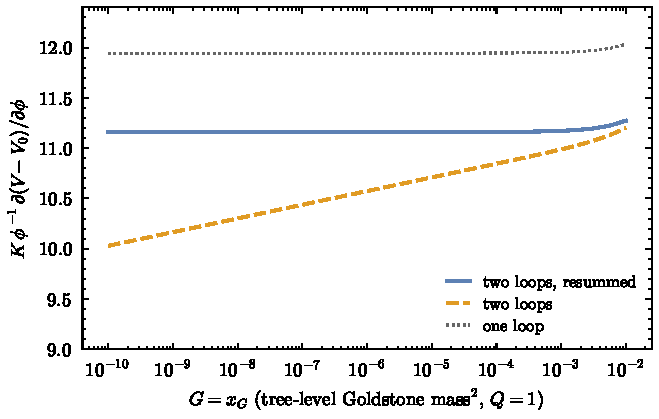
\includegraphics[width=0.72\linewidth]{../figs/goldstone.pdf}
\caption{木の最小点の近くの最小化の条件。$Q=1$ の基準点で、$K\phi^{-1}\partial(V-V_0)/\partial\phi$ を Goldstone ボソンの木の質量の2乗 $G$ の関数として描いた（$m^2$ を固定して $\phi$ を動かす）。点線は1ループ、破線は2ループ、実線は再和した2ループ \eqref{eq:vhat}。2ループの曲線は $\lambda\hat\Delta_1\ln G/K$ で発散し、再和した曲線は $G\to0$ で一定の値に近づく（\texttt{results/goldstone\_curve.csv}）。}
\label{fig:goldstone}
\end{figure}

\begin{table}[tbp]
\centering\small
\caption{$Q=2$（$e=\frac12\sqrt s$、$\lambda=\frac{25}{32}s$、$m^2=\frac{25}8$）での最小点 $v$ と最小値 $V_{\min}$（$\Lambda=0$）。再和した $\hat V$ \eqref{eq:vhat} と2ループの $V$ は数値で最小化し、条件~\eqref{eq:mincond} と式~\eqref{eq:vmin}、$\hbar$ 展開と比べた（\texttt{results/goldstone\_numeric.csv}）。最後の行は $s=\frac14$ と $\frac18$ の差の比で、左から $\hat V$ と条件、$\hat V$ と $\hbar$ 展開、2ループの $V$ と $\hat V$ の差（$v$）、$\hat V$ と $\hbar$ 展開の差（$V_{\min}$）。}
\label{tab:goldstone}
\begin{tabular}{rrrrr}
\toprule
$s$ & $\hat V$ を最小化 & 条件 \eqref{eq:mincond} & $\hbar$ 展開 & 2ループの $V$ を最小化 \\
\midrule
\multicolumn{5}{l}{$v$} \\
1 & $2.0197635988$ & $2.0197168811$ & $2.0196785261$ & $2.0198485583$ \\
$\frac12$ & $2.8421350585$ & $2.8421263927$ & $2.8421196916$ & $2.8421664283$ \\
$\frac14$ & $4.0096063101$ & $4.0096047068$ & $4.0096035288$ & $4.0096176877$ \\
$\frac18$ & $5.6636176911$ & $5.6636173959$ & $5.6636171883$ & $5.6636217742$ \\
\midrule
\multicolumn{5}{l}{$V_{\min}$（条件の列は式~\eqref{eq:vmin}）} \\
1 & $-3.1978013503$ & $-3.1976716255$ & $-3.1976888986$ & $-3.1977765293$ \\
$\frac12$ & $-6.3242244164$ & $-6.3241928651$ & $-6.3241970486$ & $-6.3242170556$ \\
$\frac14$ & $-12.5749578807$ & $-12.5749500935$ & $-12.5749511236$ & $-12.5749557727$ \\
$\frac18$ & $-25.0753298405$ & $-25.0753279055$ & $-25.0753281611$ & $-25.0753292495$ \\
\midrule
比 & $5.43$ & $5.53$ & $2.79$ & $4.02$ \\
\bottomrule
\end{tabular}
\end{table}

\paragraph{手順 (4)：背景場の $R_\xi$ ゲージと Nielsen 恒等式。}二つのスクリプトで確かめた。一つ目は \texttt{v2\_rxi\_feyncalc.wl} で、手順 (1) と同じ計算を $\xi$ を残して行った。1ループのノートの FeynRules の模型の $R_\xi$ ゲージは、$v$ を $\phi$ と読み替えると背景場の $R_\xi$ ゲージになる。Goldstone ボソンの伝播関数の質量を $Z_+$ の記号に、ゴーストとゲージ場の $\xi$ の極の質量を $\eta$ の記号に置き換え、残りの $\xi$ は $\eta/Z$ とした。真空の図は10個で、Landau ゲージと違ってゴーストの図も効く。積分族は12個、積分は39個、マスター積分は24個で、点や分子を持つものはなかった。1ループの対抗項の挿入は、裸のパラメータで書いた $V_1$~\cite{mp18} を、Martin--Patel の1ループの対抗項（$m^2$、$\lambda$、$e$、$\xi$、$\tilde\xi$、$\phi^2$）で1次まで動かしたものとした（$\tilde\xi\ne\xi$ の方向は第~\ref{sec:rxi} 節の1次の形）。極は局所的で、Martin--Patel の2ループの対抗項（$\phi^2$ の2ループの部分を含む）を入れた裸の木のポテンシャルの極とちょうど打ち消した。有限部分は式~\eqref{eq:V2rxi} と21個の単項式のすべてで記号として一致した（$I$ は7種類）。結果を \texttt{results/v2\_rxi.m} に書き出した。

二つ目は \texttt{nielsen\_rxi.wl} である。(a) 式~\eqref{eq:V2rxi} の $\xi\to0$ は式~\eqref{eq:V2} に記号として一致した。(b) 手順 (2) の $\beta$ と Martin--Patel の $\beta_\phi$、$\beta_\xi$、$\beta_{\tilde\xi}$ で、$V_0+V_1/K+V_2/K^2$ の $Q$ 依存は $1/K$ と $1/K^2$ の両方で記号として0になった。$\beta_\phi$ を Landau ゲージの $-\gamma\phi$ に替えると、$1/K$ で $\xi e^2\phi^2(m^2-\lambda\phi^2)$ が残る（1ループのノートの背景場の異常次元 $\gamma_v$ と同じ）。(c) $V_1'(v_0)=v_0[\hat\Delta_1+\lambda A(\xi Z)]$ を確かめ、式~\eqref{eq:N} の $N$ を $\xi$ で微分すると、$I$ の微分に Martin の式 (A.23) を使って記号として0になった。$\xi\to0$ の極限（$A(\xi Z)=\xi Z[\ln(\xi Z)-1]$）は Landau ゲージの $N$ に等しい。したがって背景場の $R_\xi$ ゲージでは、$\hbar$ 展開の $V_{\min}$ は $O(\hbar^2)$ まで $\xi$ によらず、式~\eqref{eq:nielsen2} が成り立つ。(d) 基準点（$Q=1$）の数値を表~\ref{tab:nielsen} に示す。$V_2(v_0)$ は $\xi=0$〜$10$ で117変わるが、$N$ は $6\times10^{-14}$ 以内で同じで、$V_{\min}=-3.112735344770952$ は手順 (3) の $\hbar$ 展開の値に等しい。最小点の1ループのずれ $v_1/K$ は $\xi$ による。$V_0+V_1/K+V_2/K^2$ をそのまま数値で最小化すると（$\xi=\frac12,1,3$）、最小値は $\hbar$ 展開と $2.7\times10^{-4}$〜$2.8\times10^{-4}$ 違い、結合を $s$ 倍するとこの差は $s^2$ で減った（$s=\frac14$ と $\frac18$ の比は3.96）。固定した次数での最小値のゲージ依存は $1/K^3$ の大きさにとどまる。一方、最小点の位置は $1/K$ の次数でゲージに依存する（$\xi=\frac12,1,3$ で $v=1.97989$、$1.98011$、$1.97808$。Landau ゲージの条件~\eqref{eq:mincond} では $1.97861$）。

\begin{table}[tbp]
\centering\small
\caption{背景場の $R_\xi$ ゲージの $\hbar$ 展開（基準点、$Q=1$、$v_0=2$。\texttt{results/nielsen\_rxi.csv}）。$N$ は式~\eqref{eq:N}、$V_{\min}=V_0+V_1/K+N/K^2$、$v_0+v_1/K$ は最小点の1ループまでの位置。$\xi=0$ は Landau ゲージ（$N$ は極限）。$N$ の $\xi$ による差は $6\times10^{-14}$ 以内。}
\label{tab:nielsen}
\begin{tabular}{rrrrr}
\toprule
$\xi$ & $V_2(v_0)$ & $N$ & $V_{\min}$ & $v_0+v_1/K$ \\
\midrule
0 & $-62.679664$ & $-108.3460115454$ & $-3.1127353448$ & $1.9757923$ \\
$\frac12$ & $-67.596278$ & $-108.3460115454$ & $-3.1127353448$ & $1.9771326$ \\
1 & $-68.457361$ & $-108.3460115454$ & $-3.1127353448$ & $1.9773755$ \\
3 & $-60.895535$ & $-108.3460115454$ & $-3.1127353448$ & $1.9753240$ \\
10 & $48.263075$ & $-108.3460115454$ & $-3.1127353448$ & $1.9551705$ \\
\bottomrule
\end{tabular}
\end{table}

\paragraph{手順 (4) の続き：Fermi ゲージ。}\texttt{fermi\_v2.wl} で確かめた。Martin--Patel の電子ファイル（\texttt{V2AH}）は、再実行のスクリプトが arXiv から \texttt{work/} に取得し、SHA-256 を確かめる（本リポジトリには含めない）。(a) ファイルの一般の $V_2$ の $\tilde\xi=\xi$ は、本ノートの図からの計算（\texttt{results/v2\_rxi.m}）に記号として一致した。Landau ゲージの形は式~\eqref{eq:V2} に、Fermi ゲージの形は一般の式の $\tilde\xi=0$ に（$Z_+^2-GZ_++\xi ZG=0$ を使って）一致した。(b) Fermi ゲージの $V_0+V_1/K+V_2/K^2$ は、$Z_\pm$ を根として微分し、$\beta_\xi=-\frac23e^2\xi/K$ と $\beta_\phi=(3-\xi)e^2\phi/K-(\frac{10}3e^4+4\lambda^2)\phi/K^2$ を使うと、$Q$ 依存が $1/K$ と $1/K^2$ で記号として0になった。$\beta_\phi$ の2ループの部分は Landau ゲージの $-\gamma^{(2)}\phi$ と同じで、$\xi$ によらない（第~\ref{sec:discussion} 節）。背景場の $R_\xi$ ゲージの $\beta_\phi$ を使うと $-4\xi e^2\phi^2(m^2-\lambda\phi^2)/K$ が残る。(c) 木の最小点の近く（$\xi=1$、$G=-10^{-2}$〜$-10^{-6}$）では、$\mathrm{Re}[f(Z_+)+f(Z_-)]$ は Espinosa--Garny--Konstandin の形と相対 $4\times10^{-3}$ から $4\times10^{-7}$ まで近づいた。一方 $\mathrm{Re}\,V_2$ は $-41.0$、$-32.7$、$-23.6$、$-13.9$、$-3.7$ と $\ln|G|$ とともに変わり続け、$G\to0$ で有限の値に近づかなかった（\texttt{results/fermi\_ir.csv}）。

(d) そこで、固定した次数のポテンシャルの実部を数値で最小化し（Martin--Patel の標準模型の数値と同じ扱い。Fermi ゲージの最小点は $G\approx-0.07$〜$-0.14$ で $Z_-<0$）、ゲージによらない $\hbar$ 展開の値（手順 (3)）と比べた（図~\ref{fig:fermi}、\texttt{results/fermi\_min.csv}）。基準点では、2ループの最小値は $\xi\le2$ で両方のゲージとも $\hbar$ 展開と $3.3\times10^{-4}$ 以内で合う（Landau ゲージの実部の最小値は $3.2\times10^{-4}$）。1ループでは差は $(1.5$〜$3)\times10^{-3}$ である。$\xi$ が大きくなると、固定した次数の値は $\hbar$ 展開から離れていく（Fermi ゲージでは $\xi\gtrsim5$、背景場の $R_\xi$ ゲージでは $\xi\gtrsim20$。Martin--Patel が標準模型で見たのと同じ傾向）。結合を $s$ 倍すると、二つのゲージの違いがはっきりする。背景場の $R_\xi$ ゲージでは差が $s^2$ で減り（$s$ を半分にするごとの比は $\xi=\frac12,1,3$ で $3.99$、$\xi=10$ で $3.95$）、$1/K^3$ の大きさである。Fermi ゲージでは差が $s$ でしか減らない（$\xi=3,10$ で比 $1.92$。$\xi=\frac12,1$ では $s$ の係数が小さく、比は $1.62$、$1.83$ と2に近づく途中）。これは、Fermi ゲージで固定した2ループの次数で最小化した値に、$O(\hbar^2)$ のゲージ依存が残ることを示す。最小点では $G$ が $1/K$ の大きさで、$V_2$ 自体が $\ln|G|$ とともに変わるので、打ち切った高次の項が $1/K^2$ の大きさで効くと考えられる。これは、Fermi ゲージで極値の値をゲージによらなくするには再和が要るという Espinosa--Garny--Konstandin~\cite{egk16} の結論と合う。

\paragraph{手順 (5)：Coleman--Weinberg の模型の次の次数。}\texttt{cw\_nlo.wl} で確かめた（\texttt{run\_cw\_check.sh}、数分）。(a) Landau ゲージの $V_2$（式~\eqref{eq:V2}）で $m^2=0$、$x_h,x_G\to0$ とし、$I(0,0,x)$ と $I(0,x,x)$ の閉じた形を入れると、$\lambda\to0$ の値は $e^6\phi^4(\frac52L^2-\frac{31}3L+\frac{71}6)$ に記号として一致した。(b) 背景場の $R_\xi$ ゲージの式~\eqref{eq:V2rxi} の $\lambda\to0$ には $I(0,Z,\xi Z)$ が一つ残る。$V_2^{(\xi)}-V_2^{(0)}-\frac32\xi e^6\phi^4(L-\frac13)(L+\ln\xi-1)$ を $\xi$ で微分すると（$I$ の微分は Martin の式 (A.23)）記号として0になり、$\xi\to0$ の値も0だった。したがって式~\eqref{eq:Pxi} が成り立つ。(c) 式~\eqref{eq:cwvmin} を $\lambda(\mu)$、$e(\mu)$、$\mu$ の関数とみて、手順 (2) の $\beta_\lambda=(6e^4-12e^2\lambda)/K-\frac{208}3e^6/K^2$、$\beta_e=e^3/(3K)$ で $\mu$ 微分すると、$\lambda=se^4/K$ として主要な次数と次の次数で0になった。(d) 式~\eqref{eq:cwR} の $\dd r_1/\dd\xi$ は、Nielsen 恒等式の予言 $2(L_0+\ln\xi+1)$ に記号として一致した。(e) $m^2=0$、$Q=1$、$\lambda=e^4/K$（$L_0=0$）で、全体の1ループと2ループのポテンシャル（$\lambda$ を含むすべての項、$I$ は TSIL）を数値で最小化し（導関数は解析的に）、式~\eqref{eq:cwvmin}、\eqref{eq:cwR} と比べた（表~\ref{tab:cw}、\texttt{results/cw\_nlo.csv}）。2ループでは、$V_{\min}$ と $R$ の次の次数の式からのずれは $e$ を半分にするごとに約 $15$ 分の1になり（次の次の次数 $(e^2/K)^2$ に対数が掛かる）、Landau ゲージと $\xi=1,3$ で同じだった。$e=\frac1{16}$ では、$V_{\min}/V_{\mathrm{LO}}-1=-7.803\times10^{-4}$ が式の $-\frac{284}9\frac{e^2}K=-7.80\times10^{-4}$ に合う。ゲージ依存は、$V_{\min}(\xi)/V_{\min}(0)-1$ が1ループの $3.3\times10^{-5}$（$\xi=1$）、$-9.8\times10^{-6}$（$\xi=3$）から2ループの $-1.5\times10^{-8}$、$2.5\times10^{-9}$ に下がった。$R(\xi)/R(0)-1$ は1ループの $1.65\times10^{-5}$、$4.95\times10^{-5}$（$\frac23\xi e^2/K$）から、2ループの $6\times10^{-10}$、$1.631\times10^{-4}$ になった。後者は $2\xi\ln\xi\cdot e^2/K$（$\xi=1$ で0、$\xi=3$ で $1.630\times10^{-4}$）に一致し、曲率の比のゲージ依存が2ループでも残ることを示す。

\begin{table}[tbp]
\centering\small
\caption{CW の模型（$m^2=0$、$Q=1$、$\lambda=e^4/K$）で、全体の2ループのポテンシャルを数値で最小化した最小値 $V_{\min}$ と曲率の比 $R$ の、次の次数の式~\eqref{eq:cwvmin}、\eqref{eq:cwR} からのずれ（\texttt{results/cw\_nlo.csv}）。最後の行は $e=\frac18$ と $\frac1{16}$ の比。}
\label{tab:cw}
\begin{tabular}{rrrrr}
\toprule
& \multicolumn{2}{c}{Landau ゲージ} & \multicolumn{2}{c}{背景場の $R_\xi$、$\xi=3$} \\
$e$ & $V_{\min}/V_{\mathrm{NLO}}-1$ & $R/R_{\mathrm{NLO}}-1$ & $V_{\min}/V_{\mathrm{NLO}}-1$ & $R/R_{\mathrm{NLO}}-1$ \\
\midrule
$\frac12$ & $9.706\times10^{-4}$ & $-4.055\times10^{-4}$ & $9.718\times10^{-4}$ & $-5.951\times10^{-4}$ \\
$\frac14$ & $6.307\times10^{-5}$ & $-2.946\times10^{-5}$ & $6.339\times10^{-5}$ & $-4.125\times10^{-5}$ \\
$\frac18$ & $4.157\times10^{-6}$ & $-2.109\times10^{-6}$ & $4.188\times10^{-6}$ & $-2.826\times10^{-6}$ \\
$\frac1{16}$ & $2.742\times10^{-7}$ & $-1.487\times10^{-7}$ & $2.768\times10^{-7}$ & $-1.919\times10^{-7}$ \\
\midrule
比 & $15.16$ & $14.18$ & $15.13$ & $14.72$ \\
\bottomrule
\end{tabular}
\end{table}

\begin{figure}[tbp]
\centering
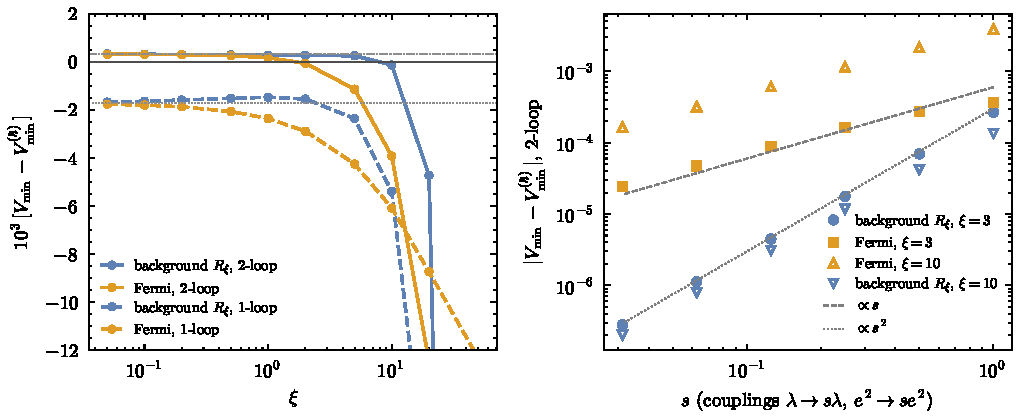
\includegraphics[width=\linewidth]{../figs/fermi.pdf}
\caption{固定した次数のポテンシャルの最小値と、ゲージによらない $\hbar$ 展開の値 $V_{\min}^{(\hbar)}$（同じループの次数）の差。左は基準点（$Q=1$）で $\xi$ の関数として描いた（実線は2ループ、破線は1ループ。青は背景場の $R_\xi$ ゲージ、橙は Fermi ゲージ。灰色の水平線は Landau ゲージの実部の最小値で、一点鎖線が2ループ、点線が1ループ）。右は2ループの差の絶対値を、結合を $s$ 倍して描いた。背景場の $R_\xi$ ゲージは $s^2$（$1/K^3$）、Fermi ゲージは $s$（$1/K^2$）で減る。}
\label{fig:fermi}
\end{figure}

\section{議論と今後}\label{sec:discussion}

\paragraph{手順 (1) で分かったこと。}Landau ゲージの $V_2$ は、Martin の一般の式に本模型の8種類の結合を入れるだけで得られ、図からの直接の計算と完全に一致した。2ループの図だけでは極に $A(x)$ や $\Aeps(x)$ を含む非局所的な項が残り、1ループのノートの Landau ゲージの対抗項（とくにゲージ場の質量の繰り込みが $Z_\Phi$ だけになること）を挿入して初めて極が局所的になり、$\Aeps$ も有限部分から消える。ゲージ場を含む図では、横波の数 $D-1$ の $\epsilon$ の部分が1ループの極と掛け合わさって $\MSbar$ に固有の有限の項（$f_{VS}$ の $2xA(y)$ など）を作る。最小点 $\phi=v$ では $x_G=0$ で $V_2$ 自体は有限だが、$x_G$ を含む項の微分は手順 (3) で扱う赤外の問題を持つ。

\paragraph{手順 (2) で分かったこと。}有効ポテンシャルの極からは、$\beta$ と場の異常次元の組~\eqref{eq:rgcomb} しか決まらない。場の異常次元を別に知るにはスカラーの自己エネルギーが要るが、本ノートではそれを計算せず、一般の式の Landau ゲージの $\gamma^{(2)}$ を使った。ゲージによらない $\beta$ と、ゲージに依存する $\gamma$ を組み合わせた値が、図の極と有限部分の両方に合ったので、両者が互いの検算になっている。一般の式を写すときの誤り（係数の写し違いや括弧の読み違い）は、標準模型の文献の値との比較で取り除いた。$V_0$ が $e$ を含まないので、$\beta_e^{(2)}$ はこの次数では検算されていない。数値では、基準点の結合と $\phi=3$ で $Q$ を2倍にすると、1ループの $V$ は4\%変わるが、2ループの $V$ と2ループの流れでは0.24\%に下がる。

\paragraph{手順 (3) で分かったこと。}Landau ゲージの Goldstone ボソンの赤外の問題は、2ループでは最小点の位置に現れる。再和しない2ループの $V$ の最小点は $1/K^2$ の大きさでずれ、基準点の $Q=1$ では最小点で $G<0$ になって $V$ が複素数になる。Martin の再和と $G$ を含まない条件~\eqref{eq:mincond} はどちらも解消し、$m^2$ を固定した $\hbar$ 展開と $1/K^3$ まで一致する。本模型の $\hat\Delta_2$ \eqref{eq:dh2} は、Martin が標準模型で求めたもの~\cite{martin14} と同じ手順で、Goldstone ボソンが1個の場合として得た。最小値 $V_{\min}$ は極値なので2ループでは赤外の問題を持たず、$\hbar$ 展開の式がそのまま使える。$V_{\min}$ は原理的にゲージによらないので、手順 (4) の Nielsen 恒等式の検算の基準になる（$v$ はゲージに依存する）。曲率は最小点で赤外の対数を持つので、スカラーの質量には極の質量が要る。

\paragraph{手順 (4) で分かったこと。}背景場の $R_\xi$ ゲージの $V_2$ は、Martin--Patel の式~\eqref{eq:V2rxi} が図からの計算とちょうど一致した。$\xi$ と $\tilde\xi$ が異なる割合で走るので、$\tilde\xi=\xi$ の $V_2$ だけでは繰り込み群の検算が閉じず、$\tilde\xi\ne\xi$ の方向の $V_1$ と背景場の異常次元（1ループのノートの $\gamma_v$ の2ループ版）が要る。1ループのノートでは極値の値 $V_0+V_1$ がゲージによらないことを見たが、2ループでは $V_2(v_0)$ 自体が $\xi$ で大きく変わり、最小点のずれの項 $-V_1'^2/(2V_0'')$ と組んで初めて $\xi$ によらなくなる（式~\eqref{eq:nielsen2}）。この打ち消しは $I$ の微分の式だけで記号として示せた。固定した次数でポテンシャルを数値で最小化すると、最小値は $1/K^3$ の大きさでゲージに依存し、最小点の位置は $1/K$ でゲージに依存する。ゲージによらない量は、$\hbar$ で展開して作る必要がある~\cite{afs15,pr11}。Fermi ゲージでは事情が違う。Martin--Patel の一般のゲージの $V_2$ は、本ノートの図からの計算と繰り込み群に整合するが、木の最小点で $V_1'$ と $V_2$ が発散するので $\hbar$ 展開そのものが作れない。固定した2ループの次数で最小化した値には $O(\hbar^2)$ のゲージ依存が残り（結合を $s$ 倍したときの差が $s$ に比例）、背景場の $R_\xi$ ゲージの $O(\hbar^3)$ より一つ低い次数から現れる。$G$ と縦波の組の $1/k^4$ の伝播関数が、最小点の近くの高次の項を $1/K$ だけ持ち上げるためと考えられ、Espinosa--Garny--Konstandin~\cite{egk16} の再和や場の再定義が要るという結論と合う。

\paragraph{手順 (5) で分かったこと。}1ループのノートでは、CW の模型の曲率の比 $V''(v)/(e^2v^2)$ に残る $\pm\frac23\xi e^2/K$ のゲージ依存は、同じ次数の2ループの項で消えると見込んだ。実際に $V_2$ を入れると、次の次数でゲージによらなくなるのは最小値 $V_{\min}$（式~\eqref{eq:cwvmin}）で、曲率の比は $\xi$ 依存の形が $\frac23\xi$ から $2\xi\ln\xi$ に変わるだけで残る（式~\eqref{eq:cwR}）。これは Nielsen 恒等式から $\dd\ln R/\dd\xi=2C'+2C/v$ として予言される量そのもので、曲率が観測量でないことの表れである。ゲージによらない質量の比には極の質量が要る。$\lambda\to0$ の $V_2$ は Andreassen--Frost--Schwartz と Espinosa--Garny--Konstandin の結果に、本ノートの模型と $\MSbar$ の規約で一致した。背景場の $R_\xi$ ゲージでは、$V_2$ の $\xi$ 依存が1ループの $\lambda\xi$ の項と最小点でちょうど打ち消し、再和は要らない。Fermi ゲージでは文献~\cite{afs15} のとおり $\lambda^{-1}e^{10}$ の daisy の図の和が次の次数に効くので、本ノートでは扱わなかった。

\paragraph{今後。}Fermi ゲージで極値の値を $O(\hbar^2)$ までゲージによらなくするには、文献~\cite{egk16} の再和や場の再定義を2ループで行う必要がある。本ノートではそこまでは扱わない。文献~\cite{lwx03} の式 (23) では、ゲージのパラメータ $\xi$ が2ループで $C_2(G)$ にだけ掛かるので、$U(1)$ の共変ゲージ（Fermi ゲージ）の $\gamma^{(2)}$ は $\xi$ によらず式~\eqref{eq:rg} と同じで、$\xi$ 依存は1ループの $\gamma^{(1)}=-(3-\xi)e^2$ だけである。これはゲージ依存が1ループで尽きるという Landau--Khalatnikov--Fradkin の変換の結果と合い、Martin--Patel の $\beta_\phi$ の $\tilde\xi=0$ の値とも一致する。次は手順 (6) の有限温度で、1ループのノートの手順 (10) で見た $\phi_c/T_c$ のゲージ依存を、次の次数までゲージによらない展開で扱う。

\appendix

\section{Landau ゲージの $V_2$ の導出}\label{app:v2}

\paragraph{一般の式の結合。}Martin~\cite{martin01} は、計量 $(-,+,+,+)$ で実のスカラー $R_i$ と実のベクトル $A^a$ の相互作用を
\begin{equation*}
-\mathcal L_S=\frac16\lambda^{ijk}R_iR_jR_k+\frac1{24}\lambda^{ijkl}R_iR_jR_kR_l,\qquad
\mathcal L_{SV}=-g^{aij}A^a_\mu R_i\partial^\mu R_j-\frac12g^{abi}A^a_\mu A^{b\mu}R_i-\frac14g^{abij}A^a_\mu A^{b\mu}R_iR_j
\end{equation*}
と書き、Landau ゲージの $\MSbar$ の $V_2$ を $V_{SSS}=\frac1{12}(\lambda^{ijk})^2f_{SSS}$、$V_{SS}=\frac18\lambda^{iijj}f_{SS}$、$V_{SSV}=\frac14(g^{aij})^2f_{SSV}$、$V_{VS}=\frac14g^{aaii}f_{VS}$、$V_{VVS}=\frac14(g^{abi})^2f_{VVS}$ の和で与える（添字はすべて和をとる。$f_{SSS}=-I$、$f_{SS}(x,y)=A(x)A(y)$、ほかは式~\eqref{eq:fs}）。本模型を背景場 $\phi$ のまわりで展開すると、$V=\frac\lambda4((\phi+h)^2+G^2)^2-\frac{m^2}2((\phi+h)^2+G^2)$ から
\begin{equation*}
\lambda^{hhh}=6\lambda\phi,\quad \lambda^{hGG}=2\lambda\phi,\quad \lambda^{hhhh}=\lambda^{GGGG}=6\lambda,\quad \lambda^{hhGG}=2\lambda
\end{equation*}
を得る。運動項 $-|D\Phi|^2=-\frac12[(\partial h+eAG)^2+(\partial G-eA(\phi+h))^2]$（計量 $(-,+,+,+)$）からは
\begin{equation*}
g^{AAh}=2e^2\phi,\quad g^{AAhh}=g^{AAGG}=2e^2,\quad g^{AGh}=-g^{AhG}=e
\end{equation*}
を得る。$-e\phi A\cdot\partial G$ の混合は横波の伝播関数と縮約して消える。和をとると、$V_{SSS}=-\frac1{12}[36\lambda^2\phi^2I(x_h,x_h,x_h)+3\cdot4\lambda^2\phi^2I(x_h,x_G,x_G)]$、$V_{SS}=\frac18[6\lambda A(x_h)^2+6\lambda A(x_G)^2+2\cdot2\lambda A(x_h)A(x_G)]$、$V_{SSV}=\frac14\cdot2e^2f_{SSV}(x_h,x_G,x_A)$（$f_{SSV}$ は前の二つの引数について対称）、$V_{VS}=\frac14\cdot2e^2[f_{VS}(x_A,x_h)+f_{VS}(x_A,x_G)]$、$V_{VVS}=\frac14(2e^2\phi)^2f_{VVS}(x_A,x_A,x_h)$ で、式~\eqref{eq:V2} になる。

\paragraph{図からの計算。}Euclid の作用で、$V_2$ は相互作用の1次の4点の項の期待値と、3点の項の2次の連結な期待値の $-\frac12$ 倍の和である。スカラーだけの図は、8の字が $\frac\lambda4\langle(h^2+G^2)^2\rangle=\frac34\lambda T_h^2+\frac12\lambda T_hT_G+\frac34\lambda T_G^2$（$T_x=\int\frac1{k^2+x}$）、日の出型が $-\frac12\lambda^2\phi^2\langle h^3h^3\rangle-\frac12\lambda^2\phi^2\langle hG^2\,hG^2\rangle=-3\lambda^2\phi^2S(x_h,x_h,x_h)-\lambda^2\phi^2S(x_h,x_G,x_G)$ である（$S$ は日の出型の積分）。ゲージ場の図では、横波の射影 $P_{\mu\nu}(k)=\delta_{\mu\nu}-k_\mu k_\nu/k^2$ の縮約 $P_{\mu\mu}=D-1$、$P(k){:}P(q)=D-2+(k\cdot q)^2/(k^2q^2)$ と、$hGA$ の頂点の $(2k+p)\!\cdot\!P(p)\!\cdot\!(2k+p)=4[k^2-(k\cdot p)^2/p^2]$ が現れる。$k\cdot q$ を伝播関数の分母で書き、$1/(k^2(k^2+x))$ を部分分数に分けると、すべての積分が $T_xT_y$ と、質量が $\{0,x_h,x_G,x_A\}$ の日の出型 $S$ に直る（手順 (1) の FeynCalc と Kira の計算はこれを自動で行う）。

\paragraph{対抗項の挿入。}裸の量を $m_0^2=(1+\delta_{m^2})m^2$、$\lambda_0=\mu^{2\epsilon}(1+\delta_\lambda)\lambda$、$\phi_0=Z_\Phi^{1/2}\phi$、$A_0=Z_A^{1/2}A$、$e_0=\mu^\epsilon Z_ee$（$Z_eZ_A^{1/2}=1$）とすると、揺らぎ $h$ の2次の項は $\frac12Z_\Phi[(\partial h)^2+x_{h0}h^2]$、$x_{h0}=-m_0^2+3\lambda_0\phi_0^2$ になる。1ループの図への挿入は $\frac12\int(\delta Z_\Phi k^2+\delta Z_\Phi x_h+\delta x_h)/(k^2+x_h)=\frac12\delta x_hT_h$（$\int1=0$）で、$\delta x_h=-m^2\delta_{m^2}+3\lambda\phi^2(\delta_\lambda+\delta Z_\Phi)$ である。$G$ も同様に $\delta x_G=-m^2\delta_{m^2}+\lambda\phi^2(\delta_\lambda+\delta Z_\Phi)$ である。ゲージ場の横波の2次の項は $\frac12[Z_Ak^2+e^2Z_\Phi\phi^2]$ なので、挿入は $\frac{D-1}2x_A(\delta Z_\Phi-\delta Z_A)T_A$ である。Landau ゲージの1ループの値を入れると式~\eqref{eq:ct} になる。$\delta_{m^2}$ と $\delta_\lambda$ はゲージによらず、$V_1$ の極を $V_0(\phi_0)$ の対抗項で消す条件 $\delta_{m^2}+\delta Z_\Phi=4\lambda/(K\epsilon)$、$\lambda(\delta_\lambda+2\delta Z_\Phi)=(10\lambda^2+3e^4)/(K\epsilon)$ を満たす。

\section{繰り込み群の関数と極}\label{app:rg}

\paragraph{ダミーのスカラー。}Luo--Wang--Xiao~\cite{lwx03} は、次元を持つパラメータの $\beta$ 関数を、伝播せずゲージの電荷も持たない実のスカラー $\phi_{\hat d}$ を加えて、4点の結合の $\beta$ 関数から読む。ポテンシャルの $\frac12m^2_{ab}\phi_a\phi_b$ は、$\phi_{\hat d}=1$ と置いた $\frac1{4!}\cdot6\lambda_{ab\hat d\hat d}\phi_a\phi_b\phi_{\hat d}^2$ と同じなので $\lambda_{ab\hat d\hat d}=2m^2_{ab}$ で、本模型では $m^2_{ab}=-m^2\delta_{ab}$ である。同様に $\Lambda=\lambda_{\hat d\hat d\hat d\hat d}/24$ である。したがって $\beta_{m^2}=-\beta_{11\hat d\hat d}/2$、$\beta_\Lambda=\beta_{\hat d\hat d\hat d\hat d}/24$ で、一般の式の内部の添字の和からはダミーを除く。たとえば1ループでは $\beta_{\hat d\hat d\hat d\hat d}=\Lambda^2_{\hat d\hat d\hat d\hat d}=3\sum_{ef}\lambda_{\hat d\hat def}^2=24m^4$ で、$\beta_\Lambda^{(1)}=m^4$ である。2ループでは、ダミーの添字を一つだけ持つ結合（3点の結合）が0なので、文献~\cite{lwx03} の式 (44) のうち $g^2(2\bar\Lambda^{2S}-6\Lambda^{2g})$ だけが残る。$\bar\Lambda^{2S}_{\hat d\hat d\hat d\hat d}=24m^4$、$\Lambda^{2g}_{\hat d\hat d\hat d\hat d}=12m^4\sum_{eg}\theta_{eg}^2=-24m^4$ から $\beta_{\hat d\hat d\hat d\hat d}=192e^2m^4$、$\beta_\Lambda^{(2)}=8e^2m^4$ である。

\paragraph{極と繰り込み群の関数。}$D=4-2\epsilon$ で $\phi_0=\mu^{-\epsilon}Z_\Phi^{1/2}\phi$ とすると、裸のポテンシャルは
\begin{equation*}
V_0^{\mathrm{bare}}=\mu^{-2\epsilon}\Bigl[R-\frac12M\phi^2+\frac14L\phi^4\Bigr],\qquad R=\mu^{2\epsilon}\Lambda_0,\quad M=m_0^2Z_\Phi,\quad L=\mu^{-2\epsilon}\lambda_0Z_\Phi^2
\end{equation*}
で、$\MSbar$ では $\ln L=\ln\lambda+l_1/\epsilon+l_2/\epsilon^2+\cdots$、$\ln M=\ln m^2+n_1/\epsilon+n_2/\epsilon^2+\cdots$、$R=\Lambda+c_1/\epsilon+c_2/\epsilon^2+\cdots$ と書ける。裸の量が $\mu$ によらないこと（$\beta_\lambda=-2\epsilon\lambda+\cdots$、$\beta_e=-\epsilon e+\cdots$、$\dd\phi/\dd\ln\mu=(\epsilon-\gamma)\phi$）から、$\epsilon$ の0次と $1/\epsilon$ の次数を比べると、$L$ ループの部分について
\begin{equation*}
2L\,l_1^{(L)}=\frac{\beta_\lambda^{(L)}}\lambda-4\gamma^{(L)},\qquad 2L\,n_1^{(L)}=\frac{\beta_{m^2}^{(L)}}{m^2}-2\gamma^{(L)},\qquad 2L\,c_1^{(L)}=\beta_\Lambda^{(L)},
\end{equation*}
2ループの2重極について $4l_2^{(2)}=(\beta^{(1)}\!\cdot\partial)\,l_1^{(1)}$、$4n_2^{(2)}=(\beta^{(1)}\!\cdot\partial)\,n_1^{(1)}$、$4c_2^{(2)}=(\beta^{(1)}\!\cdot\partial)\,c_1^{(1)}$ を得る（$\beta^{(1)}\!\cdot\partial=\beta_\lambda^{(1)}\partial_\lambda+\beta_e^{(1)}\partial_e+\beta_{m^2}^{(1)}\partial_{m^2}$）。$1/K^2$ の次数の $V_0$ の対抗項は
\begin{equation*}
\frac{c_1^{(2)}}\epsilon+\frac{c_2^{(2)}}{\epsilon^2}-\frac12m^2\phi^2\Bigl[\frac{n_1^{(2)}}\epsilon+\frac{n_2^{(2)}+\frac12(n_1^{(1)})^2}{\epsilon^2}\Bigr]+\frac14\lambda\phi^4\Bigl[\frac{l_1^{(2)}}\epsilon+\frac{l_2^{(2)}+\frac12(l_1^{(1)})^2}{\epsilon^2}\Bigr]
\end{equation*}
で、2ループの図と対抗項の挿入の極は、これの符号を変えたものでなければならない。$1/\epsilon^2$ の係数は1ループの関数だけで決まる。極~\eqref{eq:poles} の $1/\epsilon$ の係数から、$\beta_\lambda^{(2)}-4\lambda\gamma^{(2)}$ はその $\phi^4$ の項の $-16$ 倍、$\beta_{m^2}^{(2)}-2m^2\gamma^{(2)}$ は $\phi^2$ の項の $8$ 倍、$\beta_\Lambda^{(2)}$ は $\phi^0$ の項の $-4$ 倍として読める。

\paragraph{$I$ の $Q$ 依存。}太字の積分 \eqref{eq:bold} は $\mu^{4\epsilon}$ に比例するので $Q^2\partial\mathbf I/\partial Q^2=2\epsilon\mathbf I$ である。$Q^2\partial A(x)/\partial Q^2=-x$、$Q^2\partial\Aeps(x)/\partial Q^2=A(x)$ を使って $\epsilon$ の0次を比べると、$Q^2\partial I(x,y,z)/\partial Q^2=A(x)+A(y)+A(z)-x-y-z$ を得る。

\section{検算の細部}\label{app:details}

\paragraph{Minkowski の積分から太字の積分へ。}FeynArts の振幅は Feynman 則の積の $-i$ 倍で、1ループあたり $1/(2\pi)^4$ を含む。$V_2$ は真空の図の和の $i$ 倍なので、FeynArts の振幅の和の $-1$ 倍に、$(2\pi)^8$ を掛けて1ループあたり $\int\dd^Dk/(2\pi)^D$ の測度に読み替えたものである（スカラーの8の字で $+\frac34\lambda T_h^2$ になることで確かめた）。Minkowski の積分は、1ループあたり $\dd^Dk_M=i\,\dd^Dk_E$、$1/(k_M^2-x)=-1/(k_E^2+x)$ なので、二つの1ループの積は $(-iT_x)(-iT_y)=-T_xT_y$、日の出型は $i^2(-1)^3S=S$ である。$T_x=\mathbf A(x)/K$、$S=\mathbf I/K^2$ とする。

\paragraph{AMFlow の規格化。}AMFlow の積分は $J=\int\prod\dd^Dq/(i\pi^{D/2})\prod1/(q^2-x+i0)$ で、太字の積分は $\mathbf I=(-1)^3e^{2\epsilon\gamma_E}J$（$Q=1$）である（$\phi^3$ 理論のノートと同じ）。$I=\mathbf I|_{\epsilon^0}-\sum\Aeps$ とした。

\begin{thebibliography}{99}
\bibitem{ahnote} アーベル・ヒッグス模型：1ループの構造と検算（本リポジトリ \nolinkurl{models/abelian_higgs/ResearchNote/note.pdf}）。
\bibitem{env} ループ計算環境の構築記録（本リポジトリ \nolinkurl{environment/environment.pdf}）。
\bibitem{martin01} S. P. Martin, ``Two-loop effective potential for a general renormalizable theory and softly broken supersymmetry,'' Phys. Rev. D \textbf{65}, 116003 (2002), arXiv:hep-ph/0111209。
\bibitem{mp18} S. P. Martin, H. H. Patel, ``Two-loop effective potential for generalized gauge fixing,'' arXiv:1808.07615。
\bibitem{fjj92} C. Ford, I. Jack, D. R. T. Jones, ``The standard model effective potential at two loops,'' Nucl. Phys. B \textbf{387}, 373 (1992)。
\bibitem{martin14} S. P. Martin, ``Taming the Goldstone contributions to the effective potential,'' Phys. Rev. D \textbf{90}, 016013 (2014), arXiv:1406.2355。
\bibitem{eek14} J. Elias-Miró, J. R. Espinosa, T. Konstandin, ``Taming infrared divergences in the effective potential,'' JHEP \textbf{08}, 034 (2014), arXiv:1406.2652。
\bibitem{egk16} J. R. Espinosa, M. Garny, T. Konstandin, ``Interplay of infrared divergences and gauge-dependence of the effective potential,'' Phys. Rev. D \textbf{94}, 055026 (2016), arXiv:1607.08432。
\bibitem{nielsen75} N. K. Nielsen, ``On the gauge dependence of spontaneous symmetry breaking in gauge theories,'' Nucl. Phys. B \textbf{101}, 173 (1975)。
\bibitem{pr11} H. H. Patel, M. J. Ramsey-Musolf, ``Baryon washout, electroweak phase transition, and perturbation theory,'' JHEP \textbf{07}, 029 (2011), arXiv:1101.4665。
\bibitem{afs15} A. Andreassen, W. Frost, M. D. Schwartz, ``Consistent use of effective potentials,'' Phys. Rev. D \textbf{91}, 016009 (2015), arXiv:1408.0287。
\bibitem{el20} A. Ekstedt, J. Löfgren, ``A critical look at the electroweak phase transition,'' JHEP \textbf{12}, 136 (2020), arXiv:2006.12614。
\bibitem{kklp98} K. Kajantie, M. Karjalainen, M. Laine, J. Peisa, ``Three-dimensional U(1) gauge+Higgs theory as an effective theory for finite temperature phase transitions,'' Nucl. Phys. B \textbf{520}, 345 (1998), arXiv:hep-lat/9711048。
\bibitem{mv83} M. E. Machacek, M. T. Vaughn, ``Two-loop renormalization group equations in a general quantum field theory (I)--(III),'' Nucl. Phys. B \textbf{222}, 83 (1983); \textbf{236}, 221 (1984); \textbf{249}, 70 (1985)。
\bibitem{lwx03} M. Luo, H. Wang, Y. Xiao, ``Two-loop renormalization group equations in general gauge field theories,'' Phys. Rev. D \textbf{67}, 065019 (2003), arXiv:hep-ph/0211440。
\bibitem{lx03} M. Luo, Y. Xiao, ``Two-loop renormalization group equations in the standard model,'' Phys. Rev. Lett. \textbf{90}, 011601 (2003), arXiv:hep-ph/0207271。
\bibitem{tsil} S. P. Martin, D. G. Robertson, ``TSIL: a program for the calculation of two-loop self-energy integrals,'' Comput. Phys. Commun. \textbf{174}, 133 (2006), arXiv:hep-ph/0501132。
\bibitem{amflow} X. Liu, Y.-Q. Ma, ``AMFlow: a Mathematica package for Feynman integrals computation via auxiliary mass flow,'' Comput. Phys. Commun. \textbf{283}, 108565 (2023)。
\bibitem{dralgo} A. Ekstedt, P. Schicho, T. V. I. Tenkanen, ``DRalgo: a package for effective field theory approach for thermal phase transitions,'' Comput. Phys. Commun. \textbf{288}, 108725 (2023), arXiv:2205.08815。
\end{thebibliography}

\end{document}
